\documentclass{casicswhitepaper}

\newcommand{\totalRespondents}{69\xspace}
\newcommand{\totalDevelopers}{56\xspace}
\newcommand{\totalNotDevelopers}{13\xspace}
\newcommand{\totalSearchers}{55\xspace}

% Are scientists and engineers objective in their approach to finding software?
% Scientists and engineers are not objective in their approaches to finding software

% Software search is not a science even among scientists: a profile of how scientists and engineers find software

\begin{document}
\title{\vspace*{-5ex}Software search is not a science, even among scientists}
\date{\vspace*{-1ex}\dateAndVersion}
\author{Michael Hucka and Matthew J. Graham\\
\mailto{mhucka@caltech.edu},\quad\mailto{mjg@caltech.edu}\\
California Institute of Technology\\
Pasadena, CA 91125, USA}
\maketitle

\begin{abstract}
  When they seek software for a task, how do people go about finding it?  Past research found that searching the Web, asking colleagues, and reading papers have been the predominant approaches---but is it still true today, given the popularity of Facebook, Stack Overflow, GitHub, and similar sites?  In addition, when users \emph{do} look for software, what criteria do they use?  And finally, if resources such as improved software catalogs were to be developed, what kind of information would people want in them?  These questions motivated our cross-sectional survey of scientists and engineers.  We sought to understand the practices and experiences of people looking for ready-to-run software as well as people looking for source code.  The results show that even in our highly educated sample of people, the relatively unsophisticated approaches of relying on general Web searches, the opinions of colleagues, and the literature remain the most popular approaches overall.  However, software developers are more likely than non-developers to search in community sites such as Stack Overflow and GitHub, even when seeking ready-to-run software rather than source code.  We also found that when searching for source code, poor documentation was the most common reason for being unable to reuse the code found.  Our results also reveal a variety of characteristics that matter to people searching for software, and thus can inform the development of future resources to help people find software more effectively.
\end{abstract}


\section{Introduction}

Software is critical to research~\textls[-20]{\citep{stewart2013initial, howison2015software, howison2015understanding, ince2012case, morin_2012, hettrick_2014, hannay_2009, wilson_2006, katz2016report, katz2015looking}}, yet finding software suitable for a given purpose remains surprisingly difficult~\cite{howison2015software, cannata_2005, Bourne::2015, white2014nih}.  Few resources exist to help users discover options or understand the differences between them~\cite{white2014nih}.  A recent study~\cite{bauer2014exploratory} of developers at Google underscored the depth of the problem: the authors found the factor ``most disruptive to the [software] reuse process'' was ``difficulties in finding artifacts.''  In other words, \emph{even developers at Google have difficulty finding software}.

When asked, many people say they look for software by searching the Web with a general-purpose search engine such as Google~\cite{samadi_2004, umarji_2008}.  Despite its popularity, this approach suffers from significant problems: Web search can yield dozens of viable candidates---and millions of irrelevant results.  Moreover, some questions cannot be answered through Web searches without substantial additional effort, such as what are the \emph{specific} characteristics of each software tool or how do tools \emph{differ} from each other.  Many researchers also look in the scientific literature to learn what others have used for similar tasks~\cite{lawrence2015science, joppa2013troubling}.  Searching the literature can produce more relevant results and provide other information, but it suffers from limitations too: publications are static documents that may not reflect a tool's current capabilities~\cite{wren_2004}, and moreover, not all publications describe the software they use~\cite{howison2015software}.  This can happen for various reasons, such as article length limits, an expectation that software will be described in other publications, or a disinclination by researchers to describe their full software stack or workflow.  Still other methods for finding software include asking colleagues, asking on social media, searching scientific computing gateways, and more.

The difficulty of finding software and the lack of better resources brings the potential for duplication of work, reduced scientific reproducibility, and poor return on investment by funding agencies~\citep{cannata_2005, national2003sharing, crook2013learning, poisot2015best, white2014nih, niemeyer2016challenge}.  We are interested in developing better systems to help users, especially scientific users, locate software for their needs.  In order to understand the factors that influence how software users locate software, in 2015 we conducted an electronic survey involving members of numerous mailing lists in astronomy and systems biology.  Here, we report on our methods, the survey responses, and our findings.


\section{Survey design}

Our survey was designed to shed light on current practices and experiences in searching for software in two different situations: looking for ready-to-run software, and looking for software source code.  Respondents did not have to be software developers themselves (although the results show that most were).  We chose to use a Web-based survey because it is an approach that (1) is well-suited to gathering information quickly from a wide audience, (2) requires modest development effort, and (3) can produce data that can be analyzed qualitatively and quantitatively.


\subsection{Instrument development}

We developed the survey instrument iteratively.  We began with an initial version in which we posed many questions related to searching for software.  Following the practices of other surveys in computing~\cite[e.g.,][]{varnellsarjeant2015comparing, kitchenham_2008}, we designed the instrument iteratively and payed attention to the following points:

\begin{itemize}

\item Wording.  We sought to make the questions clear and unambiguous, and avoid implying a particular perspective.  We elaborated each question with explanatory text under the question itself.

\item Relevance to user's experiences.  We limited our questions to topics that could reasonably be assumed to be within the experiences of our audience.

\item Contemporary circumstances.  We tried to ground the questions by referring to real resources and specific software characteristics that we believe are relevant to computer users today.

\item Ethics.  We avoided questions that might be construed as being too personal or about proprietary policies at participants' place of work.

\end{itemize}

To help iterate on the design of the survey instrument, we performed a pilot survey with a dozen colleagues as subjects.  Based on their feedback, we removed or expanded questions as necessary to achieve the final version.  The final survey form is presented in Appendix~A.  The instrument contained a total of 22 questions (of which 18 were content questions), and included conditional branches so that the final number of questions actually seen by any given respondent depended on the answers selected to certain screening questions.  There were five main groups of questions in the survey:

\begin{enumerate}

\item Basic demographic and general information, suitable for all respondents.

\item Questions for software users who have the freedom to choose software.  This section was only shown if participants indicated that they have some choice in the software they use.

\item Questions for software developers.  This section was only shown if respondents indicated that are engaged in software development.

\item Questions for software developers who search for source code.  This was only shown if respondents indicated both that they are software developers and that they search for software source code.

\item Survey feedback.  This section sought feedback about the survey itself.

\end{enumerate}

Questions in section No.~2 aimed to establish the relative importance of different search criteria.  Those in section Nos.~3 and~4 sought to characterize the experiences of the developer.

The survey form used a mixture of four types of questions: check boxes, pull-down selection menus, two-dimensional rating grids, and short-answer input fields.  Some of the questions allowed answers on a nominal scale (for example, approaches used for finding software), some questions used an ordinal scale (for example, the importance of different considerations when looking for software), and some were open-ended questions asking for free-form text.


\subsection{Administration}

We used Google Forms~\cite{googleforms} to implement the survey instrument.  The version of Google Forms was the free edition made available by Google, Inc., as of September, 2015.  We obtained prior approval for the survey protocol from the California Institute of Technology's Committee for the Protection of Human Subjects.  The survey form itself included a Web link to a copy of the informed consent form for survey participation.  The first question in the survey provided a clickable checkbox by which subjects had to indicate they had read the informed consent form and consented to our use of their responses to the survey.  This was the only question in the survey that required a response; all other responses were optional.

We generated a URL (Uniform Resource Locator) for the survey form using Google Shortener~\cite{googl}, a service that produces shortened URLs and simultaneously provides an analytics facility tied to the URL.  On September 1, 2015, we invited participation in the survey.  As mentioned below, we advertised the survey on mailing lists and social media oriented to the astronomical and biological sciences, particularly to computational subcommunities within those domains.  Recipients were free to participate if they chose.  The introduction and instructions for the survey were brief.  Sample invitation letters are included in Appendix~B.  The survey had no express closing date.


\subsection{Sampling plan}
\label{sampling-plan}

% Where we sent it:
%   cds-all: 77
%   sbml-interoperability: 62
%   sysbio: 213 (215 total - 2 disabled addresses)
%   sbml team: 6
%   facebook astronomy group (closed list): 1487
%   ivoa mailing list: 453
%
% Total: 2298

\newcommand{\totalPotentialRecipients}{2300\xspace}
\newcommand{\totalClicks}{172\xspace}
\newcommand{\accessRate}{7.5\%\xspace}
\newcommand{\populationResponseRate}{3\%\xspace}
\newcommand{\completionRate}{40\%\xspace}

We used nonprobabilistic convenience sampling with self-selection.  We advertised the survey on electronic mailing lists oriented to the astronomical and biological sciences: the \emph{IVOA} mailing list (astronomy), a Facebook astronomy list, the mailing list \texttt{sysbio@caltech.edu} (systems biology), the forum \texttt{sbml-interoperability@googlegroups.com} (systems biology), the list \texttt{cds-all@caltech.edu} (departmental list), and our immediate work colleagues (totalling a dozen people).  Taken together, the members are a mix of staff, students, and faculty working in academia, government laboratories, and industry.

Potential biasing factors in the results include those that are common to self-selected written surveys with convenience sampling: response bias (i.e., people who responded may have different characteristics than those who did not), coverage errors (i.e., the representation of participants may not be balanced across different subcommunities), and item bias (i.e., some questions may have been skipped intentionally or unintentionally).  An additional possible source of bias is that the authors are relatively well-known within the subcommunities to which the survey was advertised, which may have influenced respondents.  


\subsection{Population sample}
\label{population-sample}

We analyzed the results obtained by December 31, 2015.  We estimate the number of potential recipients of the mail announcements to be at least \totalPotentialRecipients.  The number of completed survey forms was \totalRespondents.  As mentioned above, our survey URL was backed by an analytics facility; this provided the number of URL clicks, the referrer sources, and source geographical locations.  According to this facility, the survey form was accessed \totalClicks times.  Using these three numbers, we can calculate the following:

\begin{enumerate}[itemsep=-0.5ex]

\item \emph{Estimated access rate to survey form}: approximately \accessRate  (\totalClicks/\totalPotentialRecipients).

\item \emph{Estimated response rate}: approximately \populationResponseRate (\totalRespondents/\totalPotentialRecipients).

\end{enumerate}

Unfortunately, we cannot be certain of the actual number of recipients.  While we can determine the number of addresses we contacted, some of the addresses on mailing lists may be obsolete or unreachable, or the recipients' electronic mail systems may have filtered out the mail messages.  Thus, we can only estimate the response rate.  We revisit this topic in \ref{conclusion}.


\subsection{Analysis}

Simple descriptive statistics were performed using custom programs written in the language Python~\cite{vanRossum1991interactively, perez2011python}, version~3.4, in combination with the NumPy~\cite{vanderwalt2011numpy} package, version~1.10.4.  The figures in this paper were generated with the help of the Python library Matplotlib~\cite{hunter2007matplotlib}, version~1.5.1.


\clearpage

\section{Results: demographics}
\label{demographics}

% In the category of "other":
%
% - One person answered thus: Computing & Math Sci. (CMS), "astrophysics", "IT".  I added 1 to the count of physical sciences (the rationale being that astrophysics is a physical science) but didn't change the count of CMS because IT can be considered part of CMS at our level of granularity.
%
% - One person answered CMS, and "Pri. A&A" and "Cosmology".  I added 1 more to physical sciences for the A&A and cosmology (because they did not also select Physical Sciences, so this is a case where the count needs to be adjusted).
%
% - One person answered "Data science" but not also CMS, so I added 1 to CMS.
%
% - Two people answered "Astronomy" for "other" as well as answering "physical sciences".  We would lump astronomy under physical sciences, so it does not change the count for physical sciences.
%
% - One person answered "Aerospace Engineering (Robotics)".  I don't know where to put that one, so left it as a real "Other".

The survey included several questions to gather general demographic information about the respondents.  One of the first questions in the survey was ``What is your primary field of work?'', with multiple choices and ``Other'' as the answer options.  \fig{disciplines} shows the answer choices and the number of responses.  Of \totalRespondents respondents, 57\% identified as working in the physical sciences, 46\% in computing and maths, 28\% in biological sciences and 7\% in a range of others.  Subjects could select more than one field, and participants made use of this feature: 17 respondents selected two fields of work, six selected three fields, and one indicated four fields of work.

\begin{figure}[h]
  \vspace*{-1ex}
  \centering
  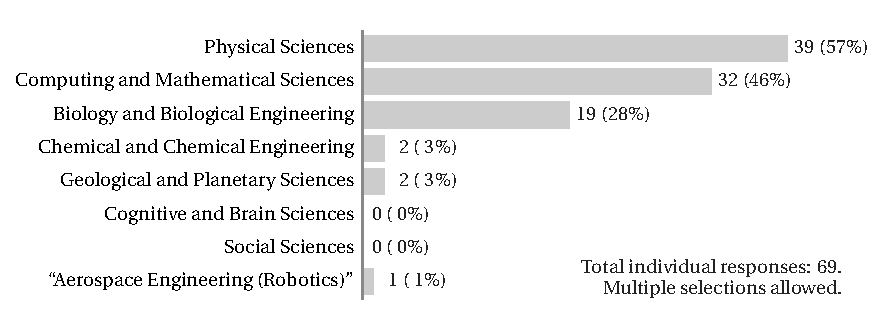
\includegraphics{files/plots/respondents-by-discipline.pdf}
  \vspace*{-3.5ex}
  \caption{Respondents by discipline.  The survey offered the first eight predefined categories and an additional slot for write-in, free-text answers.  Choices were nonexclusive.  Some respondents included write-in answers but the answers were subsumed by one of the predefined categories; in those cases, we adjusted the totals appropriately.  One response, ``Aerospace Engineering (Robotics)'', did not fit any predefined category; we included it as a true ``Other'' value.}
  \label{disciplines}
\end{figure}

To assess how computer-intensive people's work activities are, the survey included the question ``In your work, on a typical day, approximately what fraction of your time involves using or interacting directly with software on a computer or other computing device?''  The answer options were in the form of a pull-down menu with values ranging from 0\% (none) to 100\% (all), in 5\% increments.  Note the question was not limited to time spent using technical software---respondents were free to interpret this broadly to mean any software used in a work context.  \fig{time-with-software} provides a bar graph of the responses.  The results show that the overwhelming majority of our respondents spend over 50\% of their day interacting with software.  To quantify this further, assuming a typical 8~hour working day, we can conclude that 94\% of participants regularly spent more than four hours of their day engaged with software, and 68\% more than six hours.

\begin{figure}[bth]
  \centering
  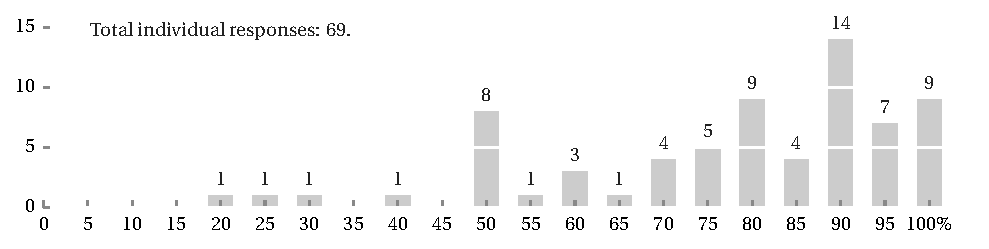
\includegraphics{files/plots/bar-graph-time-spent-with-software.pdf}
  \vspace*{-4.5ex}
  \caption{Bar graph of responses to the question ``In your work, on a
    typical day, approximately what fraction of your time involves using or
    interacting directly with software on a computer or other computing
    device?''}
  \label{time-with-software}
\end{figure}

As mentioned above, the overall motivation for the survey was to understand how people find software.  Thus, an important precondition was whether subjects actually had a choice in the software they used.  (The rationale for this is that if a person has no choice but to use software that is already provided or selected for them, then their answers to questions about how they find software would not be meaningful.)  This consideration motivated another question in the survey: ``In your work, how much freedom do you usually have to choose the software you use?''   Answers to this question were used to select subsequent survey questions: if a respondent answered ``Never'' to this question, then the remaining questions were skipped and people were shown the final survey feedback page.  \fig{freedom} provides the results for this question.  It shows that every one of our respondents had some choice in the software they used, and consequently all \totalRespondents respondents were shown the next set of questions in the survey.  %In all, 88\% of respondents said that they had \emph{some} degree of freedom to choose the software they used.

\begin{figure}[htb]
  \vspace*{1ex}
  \centering
  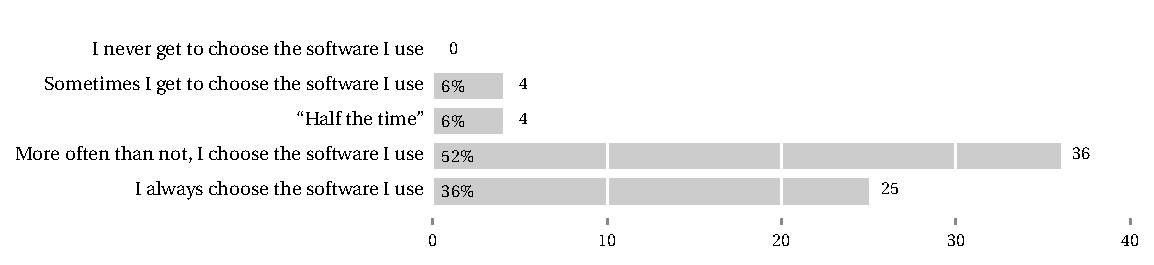
\includegraphics{files/plots/how-often-choose-software.pdf}
  \vspace*{-3.5ex}
  \caption{Responses to ``In your work, how much freedom do you usually have to choose the software you use?''.}
  \label{freedom}
\end{figure}

In response to another question, ``Are you involved in software development?'', \totalDevelopers (81\%) answered ``Yes'' and \totalNotDevelopers (19\%) answered ``No''.  The answer to this question controlled the display of an additional set of questions relevant to developers.  Among the questions that were made available to the \totalDevelopers who answered ``Yes'' were additional demographic questions.  (Those who answered ``No'' were not shown the additional demographic questions or the questions relevant to developers, and were instead taken to the final survey feedback page.)  The first question for developers was ``For how many years have you been developing software?'' with a free-form text field for answers.  We manually processed the \totalDevelopers text responses to remove extraneous text and reduce them to numbers, and then tabulated the values.  \fig{years} provides a histogram of the responses received for those who answered the question with an interpretable answer (55 out of \totalDevelopers).

% Note about the data cleaning:
% - if someone wrote "x+" or "at least x", I counted it as x.
% - if someone wrote "~x", I counted it as x.
% - one person wrote "depends on who you ask". I deleted that result.

\begin{figure}[thb]
  \vspace*{2.5ex}
  \hspace*{0.1in}
  \begin{minipage}[b]{0.265\linewidth}
    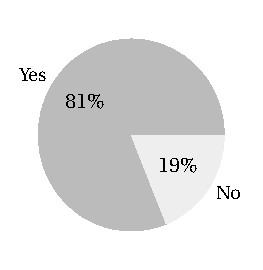
\includegraphics{files/plots/number-of-developers.pdf}
  \end{minipage}%
  \begin{minipage}[b]{0.75\linewidth}
    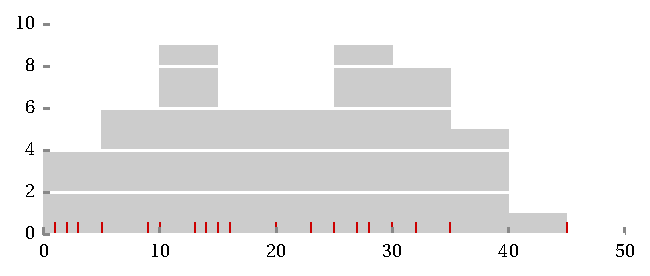
\includegraphics{files/plots/histogram-years.pdf}
  \end{minipage}%
  \vspace*{-1ex}
  \caption{(Left) Responses to the question  ``Are you involved in software development?'' (Right) Histogram plot of years that respondents have been developing software (for those who also answered ``Yes'' to the question of whether they were involved in software development).}
  \label{years}
\end{figure}

Another question asked of those who indicated they were involved in software development was ``In your current (or most recent) software development project, what is (or was) your primary responsibility?'' It offered eight multiple choice items and a ninth ``Other'' choice with a free-form text field.  The choices were nonexclusive: although we asked for people's primary responsibility, participants were free to choose more than one, and the explanatory text for the question indicated ``If it is hard to identify a single one, you can indicate more than one below.''  \fig{responsibilities} provides a tally of the responses.

\begin{figure}[thb]
  \vspace*{-1ex}
  \centering
  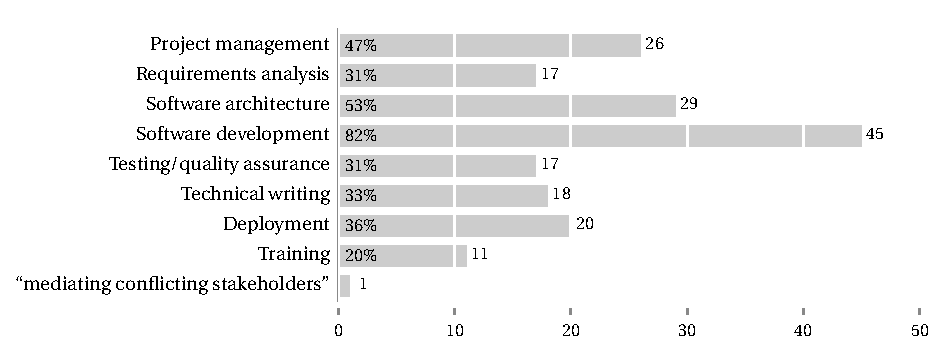
\includegraphics{files/plots/responsibilities.pdf}
  \vspace*{-3ex}
  \caption{Responses to the question  ``In your current (or most recent) software development project, what is (or was) your primary responsibility?''  This question was shown only to the 56 respondents who answered ``Yes'' to the question of whether they were involved in software development.  This survey question offered the first eight predefined categories and an additional slot for free text under ``Other''; only one respondent provide a value for ``Other''.  Choices were nonexclusive.}
  \label{responsibilities}
\end{figure}

We also asked, ``What is the typical team size of projects you are involved with?''  The form of the answers was again a set of multiple choice check boxes with an ``Other'' choice that offered a free-form text field.  Answers were provided by all \totalDevelopers respondents who answered ``Yes'' to the question of whether they were involved in software development (\fig{years}), and none of the participants selected ``Other''.  A total of 43 respondents (77\%) selected ``Small (1--5 people)'', 12 respondents (21\%) chose ``Medium (6--25 people)'', and 1 respondent selected ``Large (more than 25 people)''.

% \fig{project-sizes} provides a summary of the results.

% \begin{figure}[htb]
%   \vspace*{-1ex}
%   \centering
%   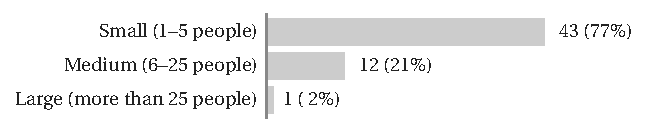
\includegraphics{files/plots/project-sizes.pdf}
%   \vspace*{-3ex}
%   \caption{Project sizes reported by the \totalDevelopers respondents who indicated they were involved in software development.}
%   \label{project-sizes}
% \end{figure}

In the final demographic question, we asked ``Which programming and/or scripting language(s) have you had the most experience with?''  This question provided 22 predefined choices along with a free-text ``Other'' option.  Choices were nonexclusive, and the elaboration under the question explicitly requested ``Please select up to 3 languages which you have used the most.''   The top five responses were: Python (selected by 59\% of participants), C (50\%), Java (34\%), shell scripting (32\%), and C++ (27\%).

These responses are consistent with expectations for the targeted scientific communities.  We expected to reach computer-literate individuals, and due to the distribution channels we used, most likely reached those working in research environments.  Languages such as Python and Java are very popular in those settings, and our survey's numbers for languages are consistent with those of a recent Stack~Overflow survey~\cite{stackexchange2016survey} for ``most popular technologies per dev type'' for their participants who chose ``Math \& Data''.  Most respondents indicated they are involved in software development, and their typical development team sizes were small, with 77\% being in groups of 1 to 5 persons.  This is common in scientific software development, especially in academia, and the fact that many respondents indicated they had multiple roles is also consistent---small teams generally require members to take on more than one role.

% 39 indicated either project mgmt or architecture or both.

Among the 81\% of the total \totalRespondents respondents who were shown this section, the median number of years of experience was 20. This suggests that the typical respondent is mid-career or part of the pre-mobile device generation.  Of these, 70\% (equal to 56\% of the overall \totalRespondents respondents) indicated that they were also primarily responsible for project management and/or software architecture, which are traditionally more senior roles.  The demographic data may thus indicate a bias in responses against more junior members of the respective communities, such as students and postdocs.  This is concerning because junior members may have different search criteria and development experiences than more experienced colleagues. The possibility should be borne in mind when interpreting the survey results in the following sections. The cause of this distribution is unknown.  We speculate that it may be due to a degree of self-selection, in that more experienced individuals are more likely to participate in community surveys.  In any case, the possible experience bias is something that future similar efforts should aim to redress.


\section{Results: how respondents find software}

The presentation of the questions in this section was triggered by a screening question asking people if they had a choice in selecting the software they used.  All respondents in our sample indicated they have some choice in the software they use, and thus all participants were shown the questions in this section.


\subsection{Ready-to-use software}
 
We first consider the search for software for a particular task rather than for development purposes. This does not imply searching for source code, and our questions emphasized that ``ready-to-run'' was the primary goal.  Note it is plausible that source code availability is still a consideration, and in the second subsection below (\sec{criteria-ready-to-use}), we seek to expose how important this criterion is.

 
\subsubsection{Approaches}
\label{approaches-ready-to-use}

\begin{figure}[b]
  \vspace*{-1ex}
  \centering
  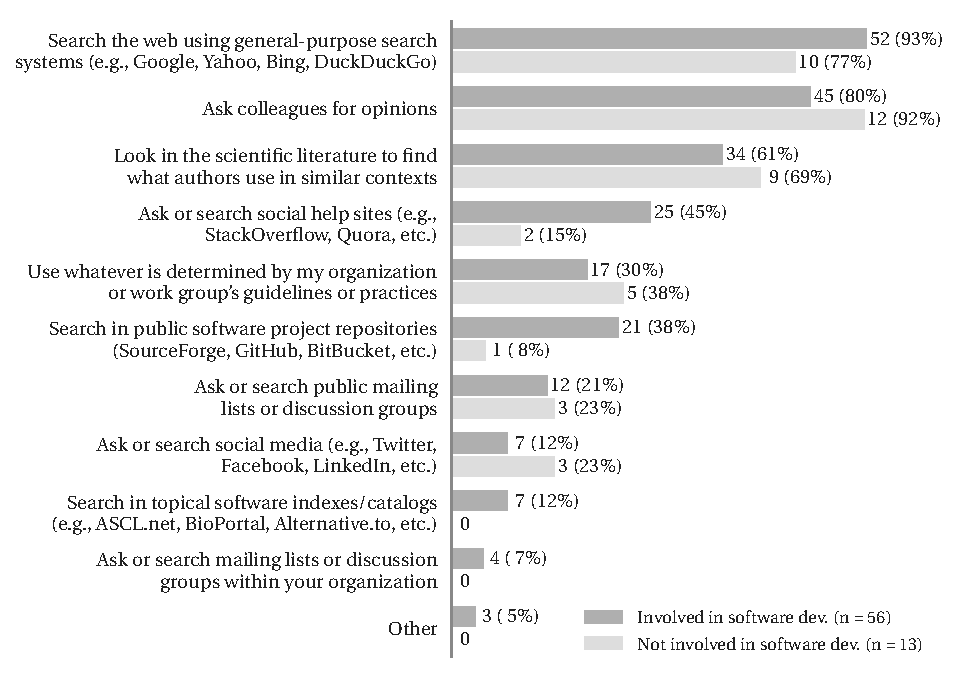
\includegraphics{files/plots/how-find-ready-to-run-v4.pdf}
  \vspace*{-4ex}
  \caption{Responses to the question ``When you need to find ready-to-run software for a particular task, how do you go about finding software?'' Answer choices were nonexclusive.  All \totalRespondents survey participants answered this question; results are subdivided according to respondents' answers to the question in \fig{years}, where \totalDevelopers people answered ``Yes'' to involvement in software development and 13 answered ``No''.  Percentages are calculated by subgroup.}
  \label{how-find-ready-to-run}
\end{figure}

To assess how people located or discovered ready-to-run software, we asked ``When you need to find ready-to-run software for a particular task, how do you go about finding software?''  The question provided multiple nonexclusive answer choices together with a free-text ``Other'' option.  The predefined answer options were developed based on our own experiences as well as similar questions posed in other surveys~\cite{sim_2011, bajrachary_2009, linstead_2009} and the results of our pilot run.  Respondents were free to choose more than one answer.  \fig{how-find-ready-to-run} summarizes the results.  We separated the responses based on how individuals answered the yes/no question about being involved in software development (\ref{demographics}).  The graph is sorted by the sum of responses across developers and nondevelopers for each answer category.

For both software developers and nondevelopers, the top three choices were (a) using general search engines, (b) asking colleagues and (c) looking in the literature.  However, developers differed from nondevelopers in their frequency of selection of these choices: the top choice for developers (93\%) was search engines, whereas for nondevelopers, it was personal recommendations (92\%).  An even larger difference is evident in the use of social help sites such as Stack Overflow, with very few nondevelopers (15\%) indicating they used this approach.  A similar difference is exhibited with respect to searching public software project repositories such as SourceForge and GitHub, with nondevelopers far less likely to indicate they use that approach.  While it is perhaps not surprising that developers would be more familiar with these resources and thus recognizing them as viable options for finding software, the results nevertheless indicate a difference in approaches used by developers versus nondevelopers.

% According to Lucian Smith: "Similarly, both subgroups rarely selected domain-specific catalogs such as ASCL.net. This last result is surprising. It may reflect ignorance ofthe existence of topical indexes, or it may reflect a belief that such resources are too narrowly focused in scope for their needs."  Another possibility is that they believe that a Google search will already utilize results from those more-specialized sites.  Certainly, I personally would never search stackoverflow directly, since when it has the appropriate response, it floats to the top of my Google results.  (Conversely, I suppose, I never find out about anything that doesn't bubble to the top of Google on its own.)  That's my own relatively unfounded assumption, at any rate.

General social media sites such as Facebook appear to be underutilized by both subsets of respondents when searching for ready-to-run software, although nondevelopers were nearly twice as likely to indicate they use these resources as a way to find software.  However, both subgroups rarely seem to use domain-specific catalogs.  This last result is surprising.  A possible explanation is that people may expect general search engines such as Google to index the domain-specific catalogs, and thus, that searching the former will subsume the latter.  This does happen in practice: results from at least some of the domain-specific catalogs can easily be demonstrated to show up in Google search outputs, though using the domain catalogs \emph{directly} will usually produce fewer, more relevant results.  A second possibility is it reflects a belief that such resources are too narrowly focused in scope for their needs.  A third possibility is that the results reflect ignorance of the existence of topical indexes.  Future research should probe this issue further and seek to understand the reasons behind this result.

Finally, the write-in answers for ``Other'' revealed a category of options we did not anticipate: all of the answers concerned the use of network-based software package installation systems such as MacPorts~\cite{fuller2002macports} and the systems available for the different Linux operating system distributions.  In retrospect, this is an obvious oversight in our list of predefined categories---the package management systems offer search capabilities, and thus, this is indeed another way for a person to find ready-to-run software.  Future surveys should include this as a predefined answer choice.


\subsubsection{Criteria}
\label{criteria-ready-to-use}

We sought to understand the selection and evaluation criteria that may come into play when users try to find ready-to-run software.  We posed the question ``In general, how important are the following characteristics when you are searching for ready-to-run software for a task?''  For the answer options, we provided a two-dimensional grid with different predefined criteria as the rows, and values on a unipolar rating scale for the columns.  The available values on the scale were ``Rarely or never important'', ``Somewhat or occasionally important'', ``Average importance'', ``Usually of above-average importance'', and ``Essential''. \fig{criteria-ready-to-run} summarizes the results.  The rows of the graph are sorted using the sum of ``Essential'' and ``Usually of above-average importance'' ratings for each criterion, to reveal the strongest preferences.  Not all participants provided a value for every criterion, which may be due either to oversight (e.g., if they did not notice they missed a row in the grid) or confusion about the instructions (if they thought they should only rate the ones they cared about).  In the discussion below, percentages in parentheses are calculated as the sum of the number of ``Essential'' and ``Usually of above-average importance'' ratings an answer received divided by the total number of responses to the question (\totalRespondents).

\begin{figure}[bht]
  \centering
  \hspace*{-1ex}%
  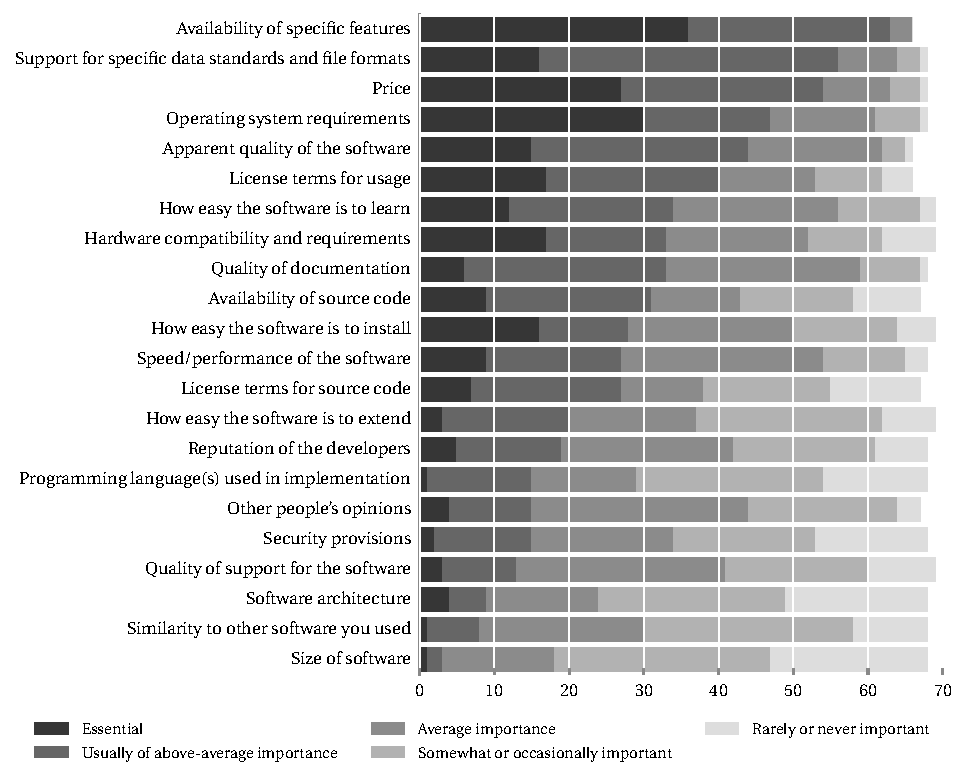
\includegraphics{files/plots/bar-graph-criteria-ready-to-run.pdf}
  \vspace*{-4ex}
  \caption{Responses to the question ``In general, how important are the following characteristics when you are searching for ready-to-run software for a task?''  All \totalRespondents respondents answered the question, but not all respondents chose to select an option for every possible characteristic.  The bar graph is sorted by the sum of the number of times the options ``Essential'' and ``Usually of above-average importance'' were selected for each characteristic.}
  \label{criteria-ready-to-run}
\end{figure}

% 2016-02-01 <mhucka@caltech.edu> In the paragraph below, I took out the part about "biological computing tends more towards the use of Windows-based systems" because my experience and that of other people I've asked is that biology is skewed towards Macs and not Windows.  But we don't need to say either way for the point to be made below, so what if we just don't mention it?  

% 2016-04-20 <mhucka@caltech.edu> I manually recalculated percentages based on the number of responses to the question (69), not the numbers per characteristic.  So for instance, for "availability of specific features", this resulted in (36 + 27)/69 = 91%.

The results show that the most important search criterion is the availability of specific features (91\%) in the software.  In fact, it was the only characteristic for which none of the respondents chose ``Somewhat or occasionally important'' or ``Rarely or never important''.  The high ranking of this characteristic is unsurprising: after all, if one is searching for software for a task, paying attention to the software's feature set is paramount.  The results show that support for specific data standards and file formats (81\%) and software price (78\%) are also major considerations, which may reflect the culture of scientific computing---software often is expected to be free, and specific areas of science often use specialized data formats (e.g, FITS in astronomy).  Operating system requirements (68\%) scored highly, while ease of usage (49\%), hardware requirements (48\%) and quality of documentation (48\%) were all ranked roughly equally.  Performance considerations (39\%) had only middling impact.

How software is implemented in terms of programming language (22\%) and the particular software architecture (13\%) were deemed relatively unimportant.  This may be simply because if one is looking for ready-to-run tools, the details of the implementation may not matter as much; it may be that other operational constraints, such as operating system support, may be more pressing constraints than how the software is written.

% related to the dominance of particular computing configurations within specific sciences.  For example, astronomical computing happens predominantly on Apple or Linux systems; in that context, 

Quality and support aspects of the software are also secondary considerations as far as information to put in a software catalog.  Both the reputation of the developer (28\%) and the level of software support (19\%) rated relatively low.  This suggests that once the software is installed, users in our sample expect that they can find their own solutions to any possible problems encountered, and that they are less concerned about future software updates. This likely reflects the culture of software use in scientific computing and how it differs from consumer or commercial environments; in the latter, software is often closed-source, licenses are purchased with implied support, and updates are expected (and often issued automatically).

A more surprising result is that other people's opinions of the software (22\%) and similarity to other software (12\%) did not rank higher.  It is possible that users resort to searching for software only when they lack other means of making selections, such as no word-of-mouth recommendations. In those cases, the approval rating of the software or its apparent familiarity may be largely ignored in favor of other criteria.  Future surveys or interviews could investigate these points more deeply.

Another surprising result is that, even though the question explicitly concerned ready-to-use software, the availability of the source code (45\%) and its licensing (39\%) were still relatively important considerations. This may reflect our particular population: a large fraction of responders identified themselves as developers. Such users are more likely to be capable and willing to alter the software to meet their specific requirements; thus, paying attention to source code and its licensing may be important for them.

It is interesting to compare these results with those of software engineering studies on desirable traits for successful open-source software projects~\cite[e.g.,][]{subramaniam2009determinants, lee2009measuring, crowston2003defining, crowston2006information, sen2012open, lee2009measuring}.  Intuitively, we expect the criteria should align: the features that people say they use to discriminate between choices when looking for software are presumably the same that differentiate successful software efforts from unsuccessful ones.  And in fact, it does turn out that code quality, documentation quality, price, and licensing terms are recognized indicators of success~\cite{subramaniam2009determinants, lee2009measuring, crowston2003defining, crowston2006information}; however, as mentioned above, our survey participants seem relatively unconcerned with developers' reputations or other people's opinions of software, which does not align with studies about traits of successful software projects.


\subsubsection{Search case histories}

To explore more deeply the topic of how users find software, we sought examples of participants' past experiences by asking an optional open-ended question: ``Please describe a past scenario when you looked for ready-to-run software.''  The survey form provided a text editing field where participants could write their responses in free-form text.  We received a total of 23 responses, of which 14 contained substantial details about the procedures or steps followed.  \fig{sample-responses} provides three examples taken from among those 14 responses.

\begin{figure}[t]
  \small
  \centering
  \fcolorbox{lightgray}{white}{\begin{minipage}{5.75in}
    \begin{center}
      --- Sample A ---
    \end{center}
    "Looked for a free UML modeler\\
    Googling for some software comparison pages\\
    Tried a few one (free or with demo license)\\
    Kept ArgoULM\\
    Not really happy with it"
  \end{minipage}}\\[-0.5ex]
  \vspace*{1.5ex}
  \fcolorbox{lightgray}{white}{\begin{minipage}{5.75in}
    \begin{center}
      --- Sample B ---
    \end{center}
"Recently I needed to find a package that would let me generate uuids in a specific language.  I wanted this to be simple (it wasn't the main point of the project, so I didn't want to reinvent-the-wheel), it ideally needed to be cross platform (testing on mac, running at scale on linux), and it needed to be something that I could install relatively quickly.\\

One large constraint was I needed to find a package that worked even on relatively out-of-date systems. This meant the newer system-packaged libraries weren't available, and trying to build them from source wasn't all that tractable (I quickly was going down a rabbit hole of other dependencies which weren't available on this old system).  So it was very difficult to find a relatively self-contained, especially when I didn't have root access.\\

My approach was to first check with package managers.  That wasn't terribly helpful, without having root access.  My next attempt was to find what would have been included on a new system (found through Googling, StackOverflow posts, man pages, etc). Then finally, I had to start searching for older versions, which were more standalone.  This final process of searching for older packages was much more random-walk googling + trial-and-error.  This last stage was probably the biggest pain.\\

(Ultimately I was able to find some software that did what I needed.)"  \end{minipage}}\\
  \vspace*{1.5ex}
  \fcolorbox{lightgray}{white}{\begin{minipage}{5.75in}
    \begin{center}
      --- Sample C ---
    \end{center}
"Looking for an authorization management software (not authentication).\\
I did some online search, plus got some info from a conference and colleagues developing one.\\
The search went on by some specific requirement about the authorization data model used by software and the interfaces available to the authorization data base.\\
Still no exact solution found.\\
One software was too complex with respect with the tasks we need and seemed to miss a top requirement (still investigating).\\
Another seems simpler but definitely lacks documentation on how to start using it."
  \end{minipage}}
  \caption{Samples of responses received to the question ``(Optional) Please describe a past scenario when you looked for ready-to-run software.''  A total of 23 survey respondents answered this question.}
  \label{sample-responses}
\end{figure}  

Analysis of all responses to this question showed that the work tasks discussed by people covered a wide range of applications, ranging from authorization management software, to statistical computing software, to visualization packages. However, the actual process described by different people was often essentially the same: firstly a broad search, usually using Google, with three to four keywords relating to functionality, implementation, and particular formats or standards, if required: e.g. ``fits viewer windows'' or ``grib format Linux''. Recommendations from colleagues can also replace the initial broad search phase. The results were reviewed on the basis of the brief descriptions returned and if one obviously met the search context then the link was followed. A typical search would follow four to five such links, and subsequent review criteria were then used to compare these. More recent software is definitely favored but many final decisions are only made when different packages have been installed and compared at a functional or operational level: ``I like to develop my own critical view by testing extensively the software.''

This anecdotal evidence is consistent with the responses to other questions in our survey. Online searches (for ready-to-use software) are primarily used to identify an initial set of candidate packages that meet a particular set of broad criteria for subsequent (offline) evaluation rather than resulting in the trusted identification of a specific match to a sophisticated query. Although this may reflect user bias, it also points to a lack of functionality in general search engines: one participant wrote ``I really miss freshmeat.net [\emph{a now-defunct software index}] because it allowed you to search for software with particular tags/keywords with particular license and language requirements. I haven't seen a good replacement for that.''

Interestingly, the reputation of the organization producing the software can result in a level of trust in the search results: ``Saw the first match ... [\emph{and}] trusted it because their employees and contractors are a large portion of the folks worldwide who work with that data format.'' The final match also does not have to be a perfect solution, as indicated by comments made in the case descriptions such as ``not really happy with it'' to ``works well enough''. This suggests a degree of pragmatism that workarounds will be found for minor issues with the identified software (see above).


\subsection{Source code}

As described in \ref{demographics}, the survey included the question ``Are you involved in software development?''  Responses to that yes/no question controlled the presentation of additional questions relevant to developers.  In that additional group of questions, one question was ``How often do you search online for software source code?'' with six answer choices that included ``Never''.  If respondents chose any option \emph{other} than ``Never'', they were shown further questions specific to searching for source code.  In this section, we discuss the results of that part of the survey.


\subsubsection{Motivations}
\label{motivations-for-src-search}

Out of \totalDevelopers participants who answered ``Yes'' to whether they were involved in software development, a total of \totalSearchers (98\% of that subset) indicated they searched for source code at least some of the time.  \fig{how-often-search-for-src} summarizes the responses received to the question ``How often do you search online for software source code?''  To help understand people's motivations for searching for software, we also asked another question: ``What are some reasons why you look for source code (when you do look)?''  Similar to other questions in the survey, it included multiple nonexclusive choices and a free-text ``Other'' field as the answer options.  \fig{why-search-for-src} summarizes the responses.

\begin{figure}[bht]
  \vspace*{-1ex}
  \centering
  \hspace*{15pt}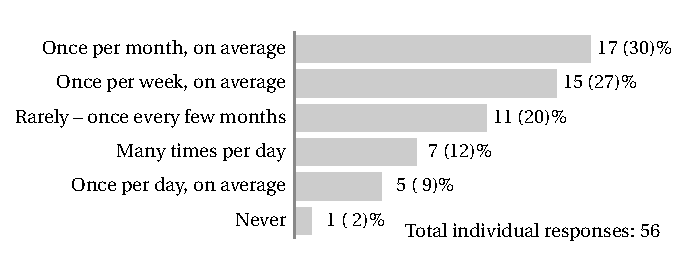
\includegraphics{files/plots/bar-graph-how-often-src.pdf}
  \vspace*{-2.75ex}
  \caption{Responses to the question  ``How often do you search online for software source code?''  Predefined answer choices were presented as the mutually-exclusive multiple choices shown on the vertical axis.}
  \label{how-often-search-for-src}
\end{figure}

\begin{figure}[hb]
  \vspace*{-0.25ex}
  \centering
  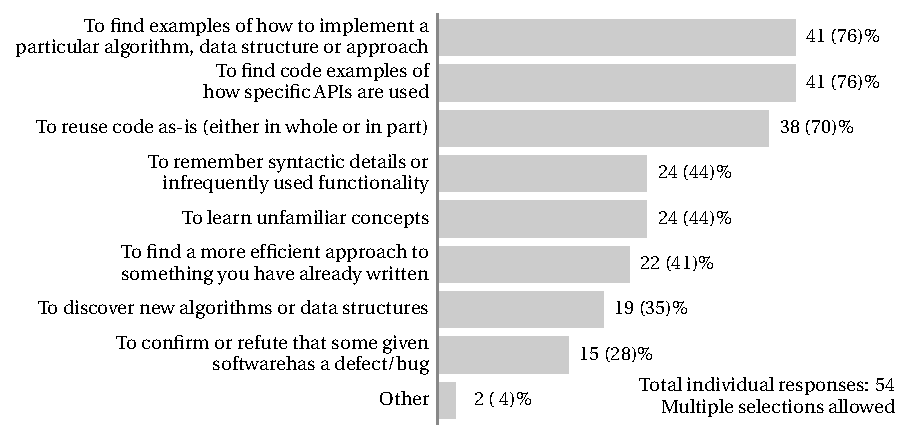
\includegraphics{files/plots/bar-graph-why-search-for-src.pdf}
  \vspace*{-1.75ex}
  \caption{Responses to the question ``What are some reasons why you look for source code (when you do look)?''  This question offered the first eight predefined categories and an additional slot for free text under ``Other''.  Answer choices were nonexclusive.  The ``Other'' results are discussed in the text.}
  \label{why-search-for-src}
\end{figure}

The results show that one in five of the developers who answered this question ($12\% + 9\% = 21\%$) are very frequent searchers, performing searches one or more times per day.  At the opposite end of the spectrum, one in five searched for source code relatively infrequently, roughly once every few months (20\%).

Seeking code examples (76\% for each of two questions) and reusing existing code as-is (70\%) were given as frequent motivations for searching.  This indicates a preference for not reinventing the wheel or, at least, a reluctance to start from an absolutely blank slate when developing.  The survey revealed that software refactoring is another common reason for searching, either to find a more efficient approach to an existing task (41\%) or to discover new algorithms and data structures (35\%). The Web is also used as an online reference source to recall syntactic details (44\%) or learn unfamiliar concepts (44\%). %\note{This is an interesting use case and one we may want to consider further when building interfaces}

Two respondents wrote answers in the ``Other'' field: ``Find software libraries to use'', and ``To understand in detail behaviour of software I'm using''.  Neither are subsumed exactly by other answer options, and indicate additional uses for software source code search that we had not anticipated.  The former answer suggests that examining other developers' code can lead to the discovery of previously unknown software libraries; this is different from searching for how specific APIs are used because it does not presuppose knowing which API library will be found or used.  The second answer suggests that another use of searching for source code is to understand detailed properties of some software, which is different from seeking to reuse code, learning how to use a specific API, or learning about unfamiliar code concepts.


\subsubsection{Approaches}
\label{approaches-find-src}

\begin{figure}[b]
  \vspace*{-2ex}
  \centering
  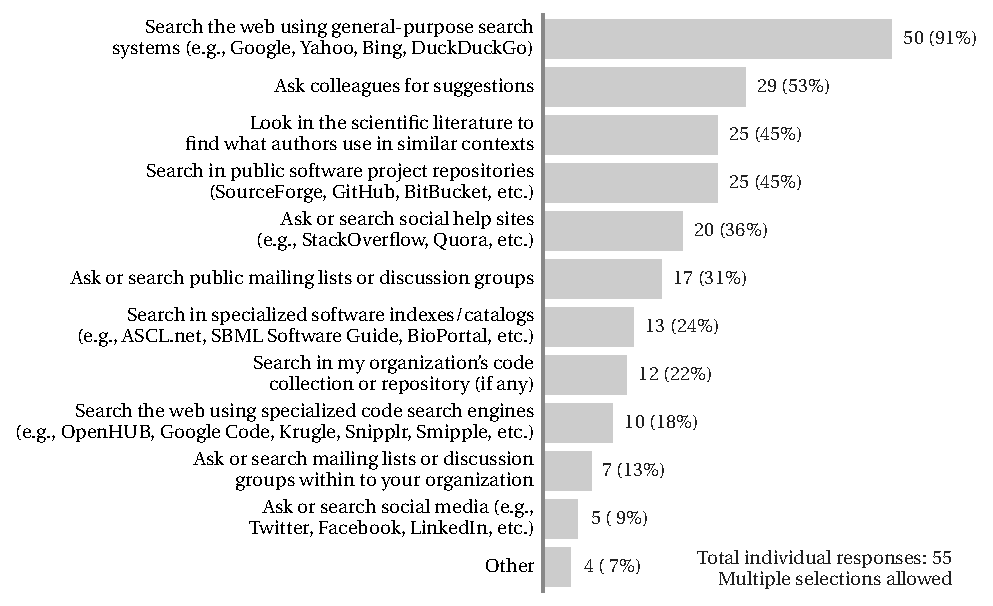
\includegraphics{files/plots/how-find-src.pdf}
  \vspace*{-4ex}
  \caption{Responses to the question ``What are some approaches you have used to look for source code in the past?''  This question offered the first eleven predefined categories and an additional slot for free text under ``Other''.  Answer choices were nonexclusive.  A total of \totalSearchers respondents answered this question.}
  \label{how-find-src}
\end{figure}

The question ``What are some approaches you have used to look for source code in the past?'' concerned the methods used by developers to find source code.  \fig{how-find-src} provides a summary of the results.  Answer options were nonexclusive multiple choices, including an ``Other'' option with a field for free-text input.  This question was answered by all \totalSearchers participants who indicated that they searched for source code at least some of the time (\fig{how-often-search-for-src}).

\begin{figure}[b]
  \centering
  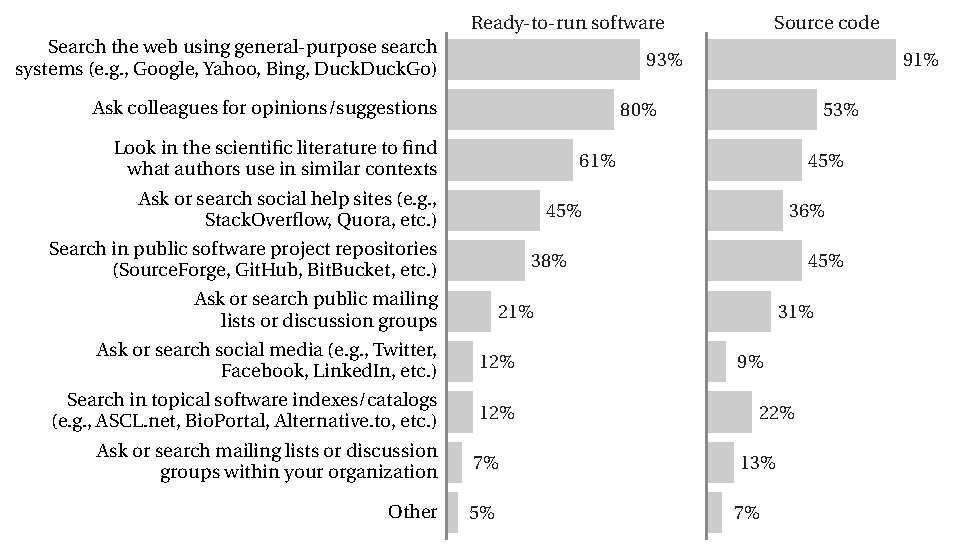
\includegraphics{files/plots/compare-how-find-v2.pdf}
  \vspace*{-1ex}
  \caption{Comparison of the results from \ref{how-find-ready-to-run} and \ref{how-find-src} for the overlapping answer categories. (Left) Subset of results from \fig{how-find-ready-to-run} for the \totalDevelopers respondents who indicated they were involved in software development.  The results have been expressed as percentages of the total number of responses for that subgroup of people.  (Right) Reproduction of the results of \fig{how-find-src}.}
  \label{compare-how-find}
\end{figure}


% 4 other write-in answers:
% "What libraries are used by other software that I like"
% "Netlib"
% "Look at the web page for that software!"
% "O'Reilly books"
%
% For analysis purposes, I think Netlib should be considered in the same
% category as ascl.net and others.

The responses to this question revealed that the use of general search engines was the most popular approach (91\%), followed by consulting colleagues (53\%), and in third place, a tie between consulting the literature and searching in repositories such as SourceForge, GitHub and BitBucket (45\% each).  The use of more specialized software indexes such as ASCL.net ranked much lower (24\%), as did searching the code collections of one's own organization (22\%).  Code search sites such as Open~Hub ranked even lower (18\%), and the use of social media systems such as Twitter, Facebook and LinkedIn ranked lower still (9\%).  Out of the four write-in ``Other'' answers, one was clearly in the same category as one of the predefined options, so we adjusted the count accordingly; the other three answers were ``O'Reilly books'', ``Look at the web page for that software!'' and ``What libraries are used by other software that I like?''  These last three represent additional approaches not anticipated in our set of predefined answer choices.

These results show that close to half of respondents search project repositories such as GitHub when looking for source code, but unexpectedly, this approach is no more popular than looking in the scientific literature.  This may reflect a population sample bias towards researchers in our study: we suspect that developers \emph{outside} of research environments are unlikely to look in the research literature as often as they search in GitHub.  On the other hand, we were surprised again at the low ranking of searching topical software indexes.

How do these results compare to those of \ref{approaches-ready-to-use}, which asked about finding ready-to-run software?  Although similar, the two questions were not identical: we offered three different answer choices because the contexts lent themselves to some different actions, and in addition, the question from \fig{how-find-ready-to-run} involved both developers and nondevelopers, whereas \emph{this} question involved only developers.  Nevertheless, we can compare the common subset of answer categories and the subset of respondents in \ref{how-find-ready-to-run} who identified themselves as software developers.  We present the results in \fig{compare-how-find}.

This shows that the top three approaches for finding \emph{both} ready-to-run software and source code are identical: searching the Web, asking colleagues, and looking in the literature.  When looking for source code, searching public repositories such as SourceForge and GitHub rises in popularity; while this is to be expected given the nature of the task and the fact that the respondents were software developers, the approach still only tied with searching the literature.  It is possible that this is again a result of our population sample consisting mainly of scientists and engineers.

Some more unexpected results reveal themselves.  First, asking colleagues for opinions is far less common when searching for source code than when searching fo ready-to-run software (53\% versus 80\%).  We have no hypothesis to explain this difference.  A second unexpected result is that the use of social help sites such as Stack Overflow was selected less frequently (36\%) when searching for source code than when searching for ready-to-run software (45\%).  Considering that Stack Overflow is one of the most popular online resources for software developers today, this result is counterintuitive.  Two possible explanations present themselves.  First, people may expect that using general-purpose search engines such as Google will return results from Stack Overflow and similar sites, and thus, they may simply not bother searching in the specialized sites directly.  A second possible explanation may come from considering responses to the question in the next section below, on the failure of past code searches: people cited an inability to find any code suitable for their purposes (69\%) and a belief that the requirements were too unique (63\%).  Perhaps these experiences and beliefs temper people's expectations of the potential for finding solutions through social help sites.  Future surveys should explore this question more deeply.

The results also show another surprising result: the use of software catalogs such as ASCL.net and BioPortal was more popular when the task was searching for source code compared to searching for ready-to-run software.  This is puzzling because the indexes do not offer source code search per se; therefore, our intuition was that the indexes would be more useful for finding ready-to-run software---but that is the opposite of what the survey revealed.  The answer must therefore lie in some other aspect of their features or their use in the context of finding source code. This is another area for future research to explore further.

Finally, we note that the use of software indexes was still quite low overall (12\% in the context of finding ready-to-run software, 22\% in the context of source code).  It ranked far lower than, for example, searching the literature, despite that software indexes are arguably much better suited to the task of finding software in a given domain or for a given purpose.  The same potential explanations we noted in \ref{approaches-ready-to-use} may apply here: namely, respondents may expect searching in Google will subsume searching in the specialized indexes, or participants may believe the indexes are too narrowly focused, or they may simply not be sufficiently aware of their existence.  More generally, this result indicates that the developers of software catalogs continue to face challenges in producing systems that users find sufficiently compelling.

% In other respects, the results in both the ready-to-run and source code cases follow largely the same trends.  The most notable difference is that searching in topical software indexes rises in popularity when searching for source code (compared to searching for ready-to-run software).  This result may reflect an incorrect belief among respondents that these indexes are specialized towards source code.  Follow-up studies could explore this topic further.

% This suggests that software development is a more subjective activity and so source code searches have a more personalized signature, determined in part by personal coding styles. (This may have implications for search anonymity issues.) This view is supported by the two main factors identified for the failure of past code searches (see below): an inability to find any code suitable for purpose (69\%) and a belief that the requirements were too unique (65\%).


\subsubsection{Reasons for \emph{search} failures}
\label{reasons-for-search-failure}

The inability to find suitable source code would hinder software reuse.  From our own experiences, we know a search for software can fail for a variety of reasons.  This motivated our inclusion of another question in the survey: ``What are some factors that have hindered your ability to FIND source code in the past?''  The question included a variety of nonexclusive predefined options, along with an ``Other'' option offering a free-text input field.  The results are summarized in \fig{factors-that-hindered}.

\begin{figure}[b]
  \centering
  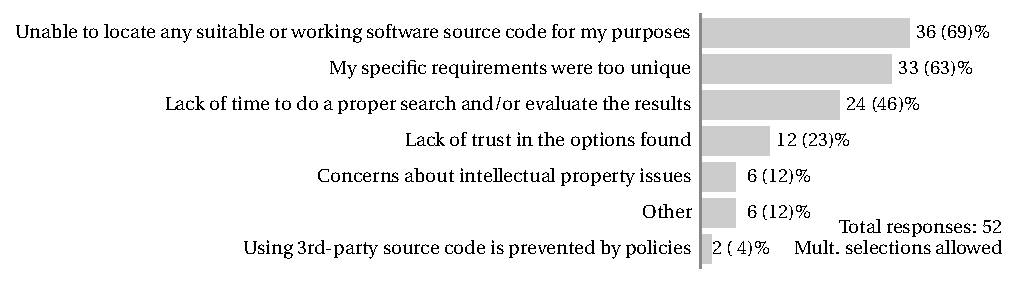
\includegraphics[width=6.5in]{files/plots/factors-that-hindered-finding-src.pdf}
  \vspace*{-4ex}
  \caption{Responses to the question ``What are some factors that have hindered your ability to FIND source code in the past?''  This question offered the first six predefined categories and an additional slot for free text under ``Other''.  Answer choices were nonexclusive.  A total of 51 survey respondents answered this question.}
  \label{factors-that-hindered}
\end{figure}

The results show that the largest hindrance is simply finding a match to one's needs, either because of difficulty finding suitable working software or because none of the options found satisfy requirements.  Time limitations also often (46\%) impact the ability to conduct proper searches for source code or to evaluate the results.  This is may be due to the large number of results that general-purpose search engines can return, which in turn may make it difficult to find suitable results easily.  (After all, the ranking systems of general-purpose search engines such as Google are optimizing for a commercial metric, such as potential advertising revenue, rather than metrics more pertinent to searching for software.)

The results also suggest that software licensing (12\%) was a minor hindrance to previous successful source code searches, even though it was a relatively important criterion for ready-to-use software (\ref{approaches-ready-to-use}), but it was a large factor (48\%) in not actually reusing the source code found (\sec{reuse-failures}). This suggests that intellectual property information is not sufficiently visible during searches.  This is consistent with the format of results presented by Google and similar general-purpose search engines: they do not usually contain license information, unless it happens to be the in the first few words of the text fragment presented as part of a given search result.


% Here are the "Other" answers:
%
% I miss freshmeat.net
% Laziness (didn't try very hard)
% Lack of proper documentation
% I'm not an expert 
% Some scientific software is hidden from search engines as authors did not bother to put it online or make a small website for it.
% Lack of documentation for evaluation of product

The write-in answers for the ``Other'' field provided additional insights into factors that contribute to being unable to locate software.  Six respondents provided ``Other'' answers; three of these were explanatory and useful in this context.  Two participants cited lack of documentation as a hindrance to either locating or evaluating software.  The third hindrance noted by a respondent was ``Some scientific software is hidden from search engines as authors did not bother to put it online or make a small website for it.''


\subsubsection{Reasons for \emph{reuse} failures}
\label{reuse-failures}

Being able to find software source code is not the only factor determining whether developers ultimately make use of the code found; other factors can hinder its use.  This motivated our survey question ``If you searched and found source code in the past, what are some factors that may have prevented you from REUSING the source code you found?''  As with most of the other questions in this survey, this one took the form of a multiple choice question with nonexclusive answer options and a free-text ``Other'' field.  We developed the multiple choice options based on our own personal experiences and feedback from the pilot survey.  \fig{hindrance-to-reusing-src} summarizes the results.

\begin{figure}[t]
  \centering
  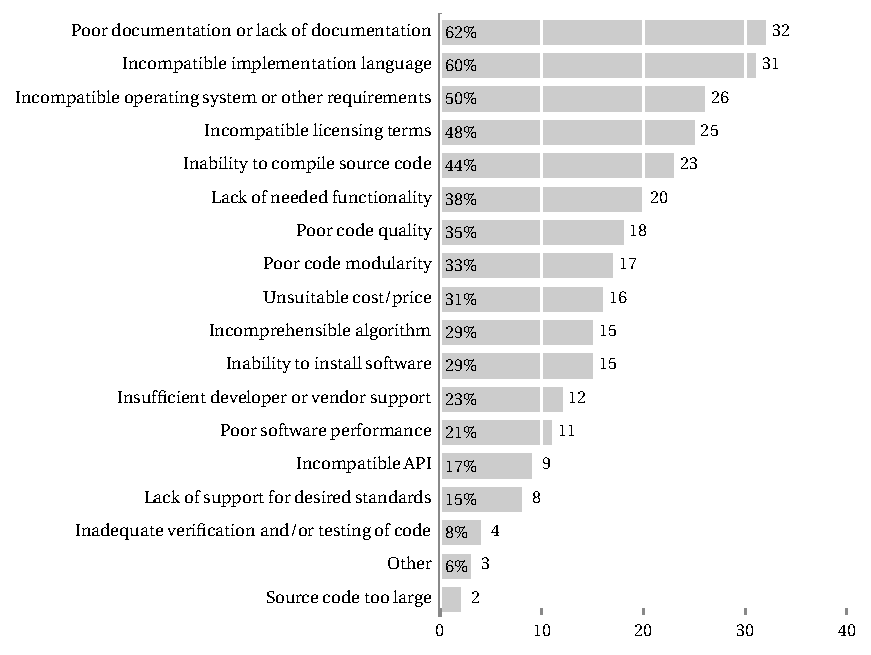
\includegraphics{files/plots/hindrance-to-reusing-src.pdf}
  \vspace*{-1.5ex}
  \caption{Responses to ``If you searched and found source code in the past, what are some factors that may have prevented you from REUSING the source code you found?''  The first 17 options were predefined; a free-text slot for ``Other'' was also provided.  Answer choices were nonexclusive.  A total of 52 survey participants answered this question.}
  \label{hindrance-to-reusing-src}
\end{figure}

The results show that the quality of the documentation (62\%) and implementation details---language (60\%) and operating system (50\%)---are the prime factors in determining whether found software will be reused. An inability to compile (44\%) the source code also appears to be a relatively common problem, although it is unclear whether this is due to issues with third-party dependencies, compiler versioning, or the actual source code itself.  Other common hindrances are discrepancies between what code purports to do (and so matches a search) and whether it actually \emph{can}: this seems to be more common with functionality (38\%) aspects than support for particular standards (15\%).

The actual quality (35\%) of the code itself, its structure (33\%), and the design of any algorithm (29\%) are less significant factors. Performance (21\%) and verifiability (8\%) are also surprisingly minor considerations to reuse, but this may be related to the didactic nature of many searches: it may not actually be that important if the code is efficient (or even fully functional) if a developer is only looking to learn something.  Finally, the level of support (23\%) for any code remains a minor factor and pricing (31\%) is also a less significant consideration than for ready-to-run software. Once code has been identified that actually meets the search parameters, it seems that developers are more willing to pay for it (presumably there may be some way to pass the costs on to end-users).


\section{Results: information desired about software}
\label{desirable-metadata}

A potential aid to finding software is a software catalog or index that classifies known software and allows people to browse and search by various criteria~\cite{marshall2006software, allen2015looking, mena2006software, katz2015catalogs, white2014nih}.  There exists a number of public software catalogs today; most such resources are domain/community-specific~\cite[e.g.,][]{nasa2016software, hempel2016xsede, darpa2015open, allen_2012, noy2009bioportal, hucka2016software, gleeson2016current, browne1995netlib, bonisch_2013}, though some general indexes also exist~\cite[e.g.,][]{blackduck2016open, freshcode2016, johansson2016alternative, sourceforge2016}.  The currently-available catalogs are highly heterogeneous in their features and the information they present to users.  To help inform the development of improved catalogs, we sought to determine what kind of information users find important to provide about software.  We posed the following question of all participants who indicated they had the freedom to choose software (not only those who indicated they developed software): ``Suppose that it were possible to create a public, searchable catalog or index of software, one that would record information about software of all kinds found anywhere.  What kind of information would you find most useful to include for each entry in such a catalog or index?''  As with most other questions in our survey, we provided answer choices as nonexclusive multiple choices, with an additional free-text option titled ``Other''.  All \totalRespondents participants to our survey replied to this question.  \fig{info-to-include} summarizes the results.  We separated the responses based on how individuals answered the yes/no question about being involved in software development (\ref{demographics}).  The graph in \ref{info-to-include} is sorted by sum of responses across developers and nondevelopers for each answer category.

\begin{figure}[t]
  \vspace*{-1ex}
  \centering
  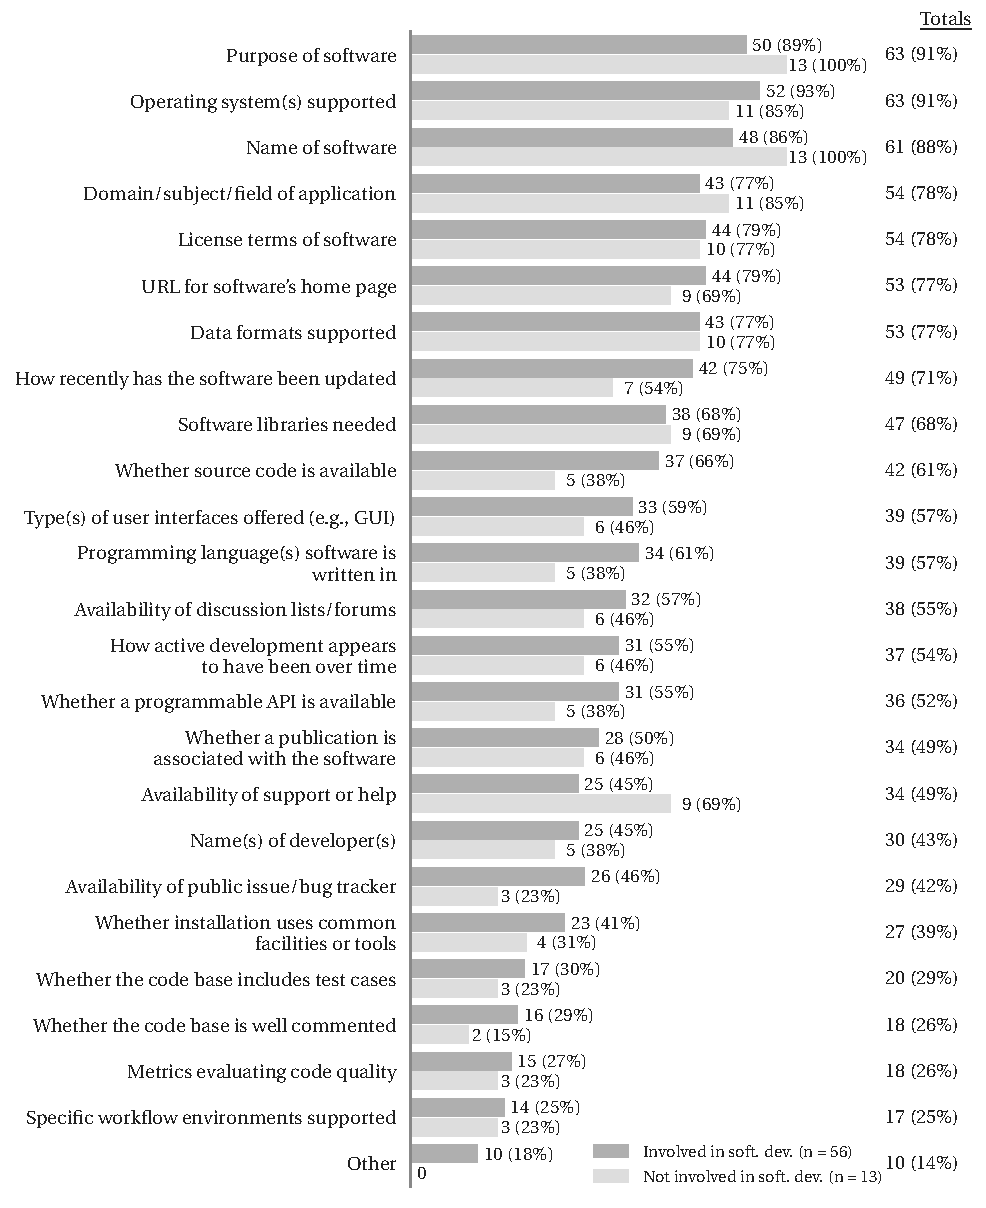
\includegraphics{files/plots/info-to-include-in-index-v5.pdf}
  \vspace*{-5ex}
  \caption{Responses to the question ``Suppose that it were possible to create a public, searchable catalog or index of software, one that would record information about software of all kinds found anywhere.  What kind of information would you find most useful to include for each entry in such a catalog or index?'' There were 24 predefined items and a slot for free text under ``Other''.  Choices were nonexclusive.  All 69 survey respondents answered this question; results are shown subdivided according to participants' answers to the question in \fig{years} (left).  The graph is sorted by totals; e.g., ``Name of software'' was the third most selected choice across both developers and nondevelopers.}
  \label{info-to-include}
\end{figure}

% Here are the values for "Other":
%   "see also"
%   URL of version control repo
%   size,price
%   whether it is packaged for Debian
%   Documentation!!!
%   Inputs needed (data, parameter format)
%   cost; stability of parent organization
%   Aprrox size of user base
%   Availability of (updated) installation instructions; Availability of plugins (list); Similar tools (list)
%   Size/nature of user base
% 
% I included the "inputs needed" as part of the count of "data formats supported" because it seems like that's what person more or less had in mind.  The rest are unique and discussed below.

When viewed across both subgroups, the five most-chosen characteristics to include were the operating system(s) supported, the purpose of the software, the name of the software, the domain of application, and license terms---all of which are very basic traits that are logically relevant to anyone looking for software.  Nondevelopers particularly favored the name and purpose as their two most-often chosen features to be included in a catalog.  (100\% of nondevelopers selected them).  After these, the next most-often chosen were a URL for a home page, the data formats supported, and how recently the software was updated.

As might be expected, more developers than nondevelopers chose availability of source code and programming language as characteristics they want to see indexed.  In other respects, the general trend for nondevelopers followed the same pattern as for developers, with one interesting exception: the availability of support or help was ranked by nondevelopers as highly as the home page URL.  By comparison, as many developers chose the availability of bug/issue trackers as often as they chose availability of support or help.  A possible explanation for this is that in the minds of developers, support options and issue trackers may be more or less synonymous, whereas nondevelopers may be less inclined to use bug trackers and more inclined to simply contact the software's support address or personnel.

Details about the software, such as the types of user interfaces offered, a programmable API, and the programming language used to implement the software, were of middle importance to survey participants.  It came as a surprise, however, that more formal indicators of software development rigor---such as test cases, well-commented code, and metrics evaluating code quality---ranked relatively low, even for developers.  We expected developers to be more discerning about the quality of software they choose.  A possible explanation is that developers may simply assume they will need to take a closer personal look at any software they choose, so they don't regard it as important to include this information in a software index.  This is another aspect of the results that would be worth investigating more deeply in future work.

Finally, ten individuals wrote additional text in the ``Other'' field of the question.  Analysis of these responses revealed that one answer was similar enough to the predefined categories that we included it in the counts shown in the graph, and one response was not interpretable.  The remaining write-in values constituted sufficiently different categories of information that they were not truly subsumed by any of the options we provided.  The following are the distinct themes that were raised in these responses:

\begin{itemize}[itemsep=-0.5ex]

\item Price (two mentions)
\item Size of the user base (two mentions)
\item Availability of documentation (two mentions)
\item Size of the software
\item Whether it is packaged for Debian
\item URL of version control repository
\item List of plug-ins available
\item List of similar tools
\item Stability of parent organization

\end{itemize}


\section{Results: survey feedback}

In the final question of the survey, we asked respondents to provide feedback on the survey itself.  The 14 comments we received were largely positive, with one or two suggestions about the survey style. Many expressed the opinion that the amount of software available in the world made the construction of a software catalog or index a difficult task but, importantly, that it would a worthwhile endeavor. A few also commented on the broader issue of searching for software, saying that ``although [they] do this quite often, [they] never really considered how or why code search succeed or not'', and the survey ``caused a bit of thinking about issues I rarely consider.'' One response was more specific on this point: ``I wasn't conscious of having explicitly searched for software for a long time. I had to think about it, but turns out I do, quite a lot---but indirectly. I don't search for software---I search for solutions. I search for information about a specific issue, using a fragment from a stack trace, a specific error code, or two or three key words to describe the issue... An indirect reference, such as a one-liner that says 'use xyz to check the status' is more likely to result in a follow up than a whole article written specifically about a product.''


\section{Related work}

As part of this project, we performed a literature survey to seek out research on topics relevant to those in our survey.  We especially sought out other work that may have surveyed how people find or discover software.  We discuss our findings in this section.


\subsection{Surveys examining how software users find ready-to-run software}

Though many surveys have examined software developers and search characteristics in the context of software \emph{code} reuse, extremely few have examined how users---whether they are developers or not---go about locating \emph{ready-to-run} software.  Our research uncovered only three reports of surveys that were not focused specifically on a software development context~\cite{joppa2013troubling, huang2013provenance, lawrence2015science}.

\citet{joppa2013troubling} surveyed 596 scientists working in a single domain (biological species distribution modeling), and asked them what software they used and why they chose that particular software.  The reasons given by the respondents provide some insight into how the scientists found the software they used, thus addressing indirectly the same topic as one of our survey questions (see \sec{approaches-ready-to-use}).  In order of most popular to least, the answers that mentioned something about ``how'' were:

\begin{itemize}[itemsep=-0.5ex]

\item ``I tried lots of software and this is the best'' (18\% of respondents)
\item ``Recommendation from close colleagues'' (18\%)
\item ``Personal recommendation'' (9\%)
\item ``Other'' (9\%)
\item ``Recommendation through a training course'' (7\%)
\item ``Because of a good presentation and/or paper I saw'' (4\%)
\item ``A reviewer suggested I use it'' (1\%)

\end{itemize}

It is interesting to note that none of the responses in Joppa et al.'s~\cite{joppa2013troubling} survey explicitly mentioned searching the Internet via (e.g.)\ a Web search engine, although it is possible that some of the answers such as ``I tried lots of software and this is the best'' and ``Other'' subsumed the use of Web searches.

\citet{huang2013provenance} summarized interviews of 15 students and faculty working in bioinformatics.  They found that four factors influenced the selection of scientific software: (1) suggestions from mentors or senior members of an institution; (2) mentor involvement in the tool's development, in cases where mentors are also developers; (3) the number of publications \emph{about} the software; and (4) the software's reputation, based on the number of publications mentioning the \emph{use} of the tool.  Unfortunately, Huang et al.'s report does not include any quantitative or qualitative data about the relative importance of these factors.

\citet{lawrence2015science, lawrence2014who} conducted a large survey in 2014 about the use of science gateways by members of scientific communities.  Their nearly 5000 respondents consisted largely of NSF-funded principal investigators, as well as members of scientific computing centers and others who expressed interest in science gateways.  Several of their questions and results are highly relevant to the topics of our own survey:

\begin{itemize}

\item They asked participants to indicate domains of expertise, and permitted multiple selections.  The top five were ``Physical and Mathematical Sciences'' (30\%), ``Life Sciences'' (22\%), ``Computer and Information Sciences'' (16\%), ``Engineering'' (16\%), and ``Environmental Sciences'' (14\%), though 16\% did not indicate a domain.  Their top three fields are thus very similar to those chosen by our survey respondents (see \fig{disciplines}), though the proportions of the three are different.

\item They asked how people learn about and choose gateways---a question closely related to our own survey's question about finding software (see \sec{how-find-ready-to-run}).  They found that 78\% indicated they learned about technologies from colleagues, 61\% indicated conferences and other meetings as a source, 51\% said publications, 38\% said Web searches and speciality sites, 33\% from students, and less than 10\% from mailing lists or other methods such as magazine advertisements.

\item They asked participants about the types of Web-based resources that were important to their work from the perspective of researchers and/or educators.  The form included a matrix of ten predefined options and five-term rating scale (``Very important'', ``Somewhat important'', etc.).  The five highest rated resources where: ``Data collections'' (75\% indicated somewhat or very important), ``Data analysis tools, including visualization and mining'' (72\%), ``Computational tools'' (72\%), ``Tools for rapidly publishing and/or finding articles and data'' (69\%), and ``Educational tools'' (67\%).

\item In another question, Lawrence et al.~\cite{lawrence2015science} asked participants ``Assuming cost is not a factor, what are the most important factors you consider when adopting a new technology? Please select the three (3) most important factors in your decision-making process''.  Since this question had direct relevance to two of our survey's questions (see \fig{criteria-ready-to-run} and \fig{info-to-include}), we include the full response results here:

\begin{itemize}[itemsep=0.2ex]
\item ``Documentation available'' (49\%)
\item ``Ability to Adapt/Customize'' (35\%)
\item ``Demonstrated Production-Quality Reliability'' (31\%)
\item ``Availability of Technical Support'' (30\%)
\item ``Open Source'' (27\%)
\item ``Existing User Community'' (20\%)
\item ``Interoperability with Other Systems'' (20\%)
\item ``Availability of Support for Bug Fixes \& Requests'' (19\%)
\item ``Testimonials/User Ratings'' (16\%)
\item ``Project Longevity'' (13\%)
\item ``Licensing Requirements'' (12\%)
\item ``Availability of Long-Term Maintenance'' (11\%)
\item ``Reputation of Those Who Built the Software'' (11\%)
\end{itemize}

\end{itemize}

The last outcome summarized above from Lawrence et al.'s survey~\cite{lawrence2015science} is surprisingly different from the results of a similar question in our survey.  Comparing the results above to our \fig{criteria-ready-to-run}, neither the relative ordering of the chosen criteria, nor the absolute positions, are consistent between the two sets of survey responses.  The differences are puzzling.  While it is true that our survey included many more possible criteria, and in addition, some criteria in Lawrence et al.'s survey question were coarser in detail, many items in both surveys are comparable, so these two differences alone are unlikely to explain the results.  It is possible that the rankings are influenced by the different answer formats: we asked participants to rank the importance of each criterion, while Lawrence et al.\ asked respondents pick their top three criteria.  In an effort to assess whether this is a possible cause, we reanalyzed our results by ranking the responses based on the sum of the number of times ``Essential'', ``Usually of above-average importance'', and ``Average importance'' were selected for each criterion.  The results are shown in \fig{criteria-ready-to-run-reranked}.  Now the quality of documentation is sixth highest in rank, and quality of the software is fourth highest, which begins to approach the high ranks these two criteria had in Lawrence et al.'s survey.  However, other features remain quite different in rankings between the survey results.

\begin{figure}[t]
  \vspace*{1ex}
  \centering
  \hspace*{-1ex}%
  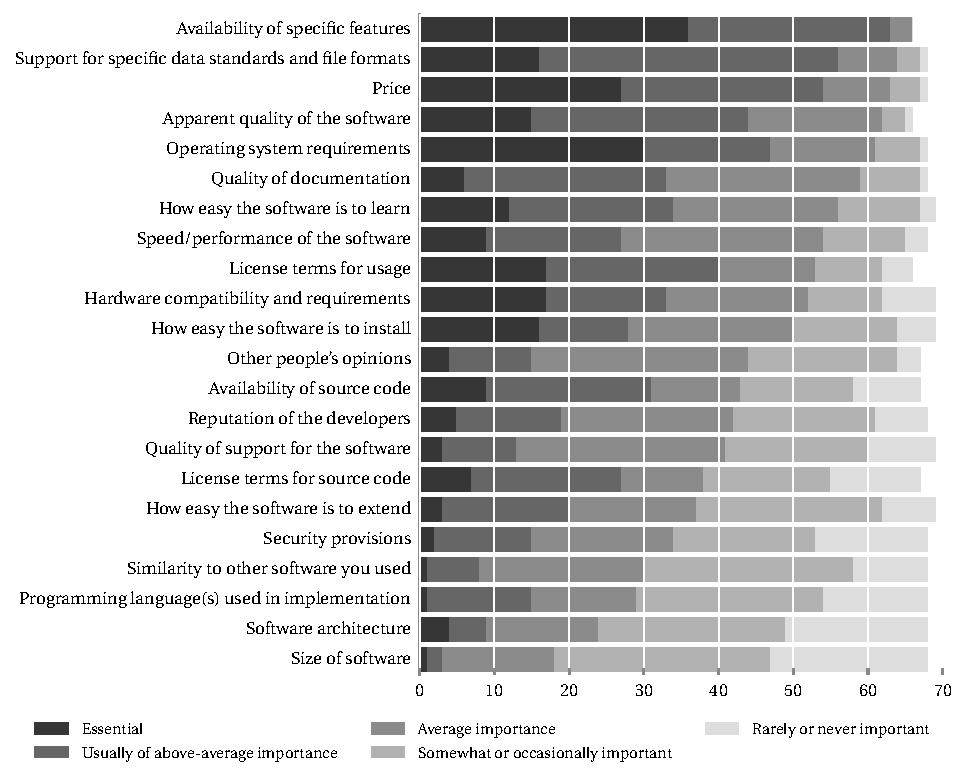
\includegraphics{files/plots/bar-graph-criteria-ready-to-run-reranked.pdf}
  \vspace*{-4ex}
  \caption{Reanalysis of the responses to the question of \protect\fig{criteria-ready-to-run}.  In this bar graph, we sorted the possible criteria by the sum of the number of times the options ``Essential'', ``Usually of above-average importance'' and ``Average importance'' were selected for each one.}
  \label{criteria-ready-to-run-reranked}
\end{figure}

Other factors therefore must be responsible for the differences in results between our survey and that of Lawrence et al.~\cite{lawrence2015science}.  We hypothesize two possibilities.  First, the context of their survey was scientific computing gateways, whereas our survey was not focused on this and considered people working with any kind of software environment.  This may influence the criteria people use to select between software options.  Second, Lawrence et al.'s survey had far more respondents than we did.  It is possible that our results for this question would be different if we had a larger sample.


\subsection{Surveys examining how developers reuse software}

% It is important to keep in mind that the approaches used by developers in these situations will likely be different from those used by end users to find software, both because developers are known to use different strategies~\cite{} and because are likely to be considering different characteristics (e.g., APIs).  Nevertheless, such studies are related to our survey.

Most studies of how users find software have done so in the context of software development and the reuse of software code.  The types of reuse in these situations range from black-box reuse of libraries or other software components (i.e., reusing code ``as-is''), to reuse of code fragments; in addition, in programming contexts, many studies examined the reuse of other kinds of artifacts such as documentation, specifications, architectural patterns, and more.  For the purposes of this review, we discuss general studies about code reuse in this section, and leave those specifically about code search to \ref{code-search-by-developers}.

One of the earliest surveys of software developers in the context of software reuse was published by Frakes and Fox~\cite{frakes1995sixteen}.  In their 1991--1992 survey of 28 U.S. organizations, they received responses to 16 questions from 113 people about questions ranging from programming language and tool preferences to the impact of legal issues.  Several results from this survey are relevant to the topics of our own survey:

\begin{itemize}

\item They found that reuse is more common in some industries than others.  The subjects in Frakes and Fox's study~\cite{frakes1995sixteen} mostly came from high-technology sectors such as the software industry, aerospace and telecommunications.  The authors found significant differences in the reuse of artifacts between different industries, as well as the types of artifacts that were reused.  The telecommunications industry had the highest level of reuse and had the aerospace the lowest.

\item They did not find that having a repository improved reuse.  Frakes and Fox reported that ``organizations with a repository have median code reuse levels 10 percent higher than organizations that do not have reuse repositories, but this difference is not statistically significant at the 0.05 level.''

\item The authors also examined whether company, division or project sizes were predictive of systematic reuse in an organization.  They found no significant correlation between reuse levels and sizes.

\item On the topic of whether participants prefer to develop their own software versus reusing someone else's, Frakes and Fox found that most of their respondents (72\%) did not have a ``not invented here'' mentality---most developers prefer to reuse when possible.

\item Several of the questions concerned factors that may or may not affect reuse behavior.  We can summarize their results as follows: CASE (Computer Aided Software Engineering) tools do not promote reuse; education about reuse practices improves the level of reuse in an organization; reuse is higher in organizations having a process that promotes reuse;  recognition for practicing reuse does not increase reuse by individuals, but monetary rewards do; and satisfaction with the quality of reusable artifacts did not affect reuse levels among the participants (but this was because the level of quality they encountered had been adequate).

\end{itemize}

\citet{samadi_2004} reported preliminary findings from a 2004 survey conducted by the NASA Earth Science Software Reuse Working Group. Their survey was distributed to government employees and contractors in the Earth science community, and asked about people's recent reuse experiences and community needs.  Several results from the study are pertinent to our work:

\begin{itemize}

\item On the topic of how people found reusable software artifacts, the following approaches were noted: (1) word of mouth or personal experiences from past projects, (2) general Web search engines (e.g., Google), (3) catalogs and repositories.  The authors report ``Generic search tools (such as Google) were rated as somewhat important, whereas specialist reuse catalogs or repositories were not cited as being particularly important''.

\item As far as criteria used to decide which specific components to choose, the authors report that ``most respondents chose saving time/money and ensuring reliability as their primary drivers for reuse''.  Further, the following additional considerations were noted: (1) ``ease of adaption/integration'', (2) availability of source code'', (3) ``cost of creating/acquiring alternative'', and (4) ``recommendation from a colleague''.  The authors further report that (a) availability of support, (b) standards compliance, and (c) testing/certification, were ``not ranked as particularly important''.

\item On the topic of barriers to reuse, two common types of barriers emerged: (1) if available software did not meet a person's specific requirements, and (2) if a given software artifact was ``difficult to understand or poorly documented''.

\end{itemize}

The last result above from \citet{samadi_2004} matches the results of our survey.  For our question about what factors hindered people from finding software (\ref{reasons-for-search-failure}), the most popular reason was finding a match to one's needs, and for our question about what hindered people's ability to reuse source code found (\ref{reuse-failures}), quality of documentation was the most popular reason.

The study was reprised in 2005 with a wider audience that included members of academia.  The results of 100 responses they received are summarized by \citet{marshall2006software}.  According to Marshall et al., the larger 2005 survey produced essentially similar results to the preliminary 2004 survey.  They noted the following:

\begin{itemize}

\item The primary reason given by people for not reusing software from outside of their group was that ``they did not know where to look for reusable artifacts and they did not know suitable artifacts existed at the time.''

\item For those who did engage in reuse, ``personal knowledge from past projects and word-of-mouth or networking were the primary ways of locating and acquiring software development artifacts.''  

\item On the topic of how people located software, the results reported by \citet{marshall2006software} seem to be inconsistent.  The authors noted that ``Web searches were of average importance while serendipity and reuse catalogs or repositories were rated the lowest''; however, in another section of the survey dealing with how to increase reuse within the Earth science community, one of the top three factors was ``having an Earth science catalog/repository for reusable artifacts.''  In other words, catalogs were rated low in one part of the survey but high in another part.  Despite this, among their conclusions, Marshall et al. noted ``the use of reuse catalogs and repositories was rated the most important method of increasing the level of reuse within the community.''

\end{itemize}

In a different NASA-centered study, Orrego and Mundy~\cite{orrego_2007_study} examined software reuse in the context of flight control systems at NASA's Independent Verification \& Validation (IV\&V) Facility.  They studied 63 projects using interviews, surveys and case studies.  In interviews with 15 people, they found that black-box reuse and other types of reuse did occur, and the degree to which a given project reused software ranged from 0\% to 80\%.  The difficulty of assessing the characteristics of software was stated as the most problematic aspect of reusing software, usually because of inadequate documentation for the software components to be reused.  Unfortunately, the Orrego and Mundy did not report the specific approaches attempted by people to locate software.

Singer et al.~\cite{singer2014software} examined how software developers active on GitHub use Twitter.  They conducted an initial exploratory survey with 271 GitHub users (270 of whom said they develop software) and followed it up with a validation survey involving 1,413 GitHub users (1,412 of whom said they develop software).  Their results have the following relevance to the topic of how people find and choose software:

\begin{itemize}

\item Developers increase their awareness of people, trends and practices by subscribing to Twitter accounts by (a) individual developers as well as software project news channels relevant to their work, (b) news services or news curators, (c) ``thought leaders'' or experts in different subject areas.  

\item Developers extend their knowledge of software (including new software tools and components) by asking and answering questions, participating in conversations, and following experts.  This can lead to serendipitous discovery of reusable methods, software components and software tools.  Singer et al. noted ``Some developers mentioned that Twitter helps them find and learn about things that they would not have been able to search for themselves, such as emerging technologies that are too new to appear in web searches.''

\end{itemize}

\citet{bauer2014exploratory} describe a study of reuse practices by developers at Google.  Despite the nature of Google as one of the preeminent software organizations today, it is surprising that there is no centrally-controlled mandate about reuse of software.  The question of what to reuse, and how, is left to engineers and managers.  (There are core libraries and software components that get reused company-wide; these are under the care of dedicated teams, but the decision of what to use for a given task or application is evidently up to individuals and product teams.)  Several of the questions in Bauer et al.'s survey~\cite{bauer2014exploratory} are relevant to the present study.

\begin{itemize}

\item They asked subjects for their top three ways of sharing software components.  They received 63 responses: common repository (97\%), packaged libraries (34\%), tutorials (31\%), blogs (19\%), email (9\%), ``I do not share artifacts'' (3\%), and ``other'' (3\%).

\item Bauer et al.\ asked about the preferred ways to find reusable software.  They received 106 responses: code search (77\%), communication with colleagues (64\%), Web search (49\%), browsing repositories (41\%), browsing documentation (23\%), ``other'' (8\%), ``code completion'' (5\%), code recommendation systems (3\%), and tutorials (3\%).  It is worth noting that Google has a centralized code repository where most of the code is available for all projects; this repository system features a centralized code search facility.

\item They also asked ``What do you do to properly understand and adequately select reusable artifacts?'' and received 115 responses: interface documentation (72\%), examples of usage on blogs and tutorials (64\%), reviewing implementations (64\%), reading guidelines (51\%), exploring third-party products (28\%), ``other'' (10\%), and participating in training for third-party products (5\%).

\end{itemize}

A final study relevant to this topic is the work of Lawrence et al.~\cite{lawrence2015science, lawrence2014who}, discussed in the previous section.  An additional question in their survey is relevant in the context of software search and reuse by developers.  They asked software developers ``How do you keep up to date with web-based technologies?'', limiting answers to two choices from a predefined list and a free-text ``Other'' field.  The three most popular answers were: using online communities via email or Web-based forums (47\%), one's own development team (43\%), and focused workshops (18\%).


\subsection{Surveys examining code search by developers}
\label{code-search-by-developers}

It has been long known from studies of developers at work~\cite[e.g.,][]{singer1997examination} that search is always a common activity.  A number of studies have also examined more specifically how developers use search to discover software.  It is important to keep mind, however, that while they are relevant to the general question of how users find software, such studies presuppose an answer: the users are \emph{performing search} on a computer, and not (say) reading papers or asking colleagues for recommendations.  Thus, the studies have a narrower scope than our survey, both in terms of the populations studied and in terms of approaches to finding software.  On the other hand, they can delve more deeply into the details of how, where, when, and why the subjects searched for software.

Umarji et al.~\cite{umarji_2008, umarji_2013} surveyed Java programmers in 2006--2007 to understand how and why they searched for source code.  Using invitations to mailing lists and newsgroups, they solicited participation to fill out a Web survey, and received 69 responses.  In the 2008 paper and the 2013 book chapter, they focused on one of the survey questions asking people to describe 1--2 scenarios in which they looked for source code on the Internet.  (A similar but earlier study by Sim et al.~\cite{sim_1998} predated the common use of Internet search for code; it has less relevance to the present work, so we do not report on it here.)  Several facets of the Umarji et al.\ study are especially relevant to our own survey:

\begin{itemize}

\item With respect to why developers searched, out of a total of 51 searches described, Umarji et al.~\cite{umarji_2008} found that the largest fraction were concerned with finding either (a) reusable code (67\% of the 51 results), (b) reference examples (33\%), or debugging activities (10\%).  Within the reuse category (a), the authors identified four themes: (1) search for code fragments; (2) search for subsystems that implemented reusable data structures, algorithms, or other elements that could be incorporated into an implementation; (3) search for packages or API libraries; and (4) search for stand-alone tools or systems (in the words of a participant, ``big piece of code that does more or less what I want'').  Within the category of reference examples (b), Umarji at al. also identified four (different) themes: (1) search for code fragments that illustrate syntax; (2) search for implementations of data structure, algorithm or widgets in order to verify a programmer's own approach or use as a basis for reimplementation; (3) search for examples of how to use a library; and (4) search for similar software to generate new ideas.  Within the category of debugging (c), developers searched for solutions to software defects (``patches'') or explanations for the cause of an error.

\item Umarji and Sim~\cite{umarji_2013} report that common starting points for searches were: (1) recommendations from friends, and (2) reviews, articles, blogs and social tagging sites.

\item With respect to how developers conducted searches, the participants in the survey used the following, in order of popularity: (1) general-purpose search engines (87\% of participants), (2) personal domain knowledge (54\%), (3) project hosting sites such as SourceForge.net~\cite{sourceforge_1999} (49\%), (4) references from peers (43\%), (4) mailing lists (23\%), and (5) code-specific search engines such as Google Code Search~\cite{googlecodesearch_2006} (16\%).

\item With respect to the selection criteria used by developers to choose a solution, Umarji and Sim~\cite{umarji_2013} report that the most important factors were: (1) software functionality (78\%), (2) type of software license (43\%), (3) price (38\%), (4) amount of user support available (30\%), and (5) level of project activity (26\%).

\end{itemize}

Gallardo-Valencia and Sim~\cite{gallardo2011kinds} examined the Web search behaviors of 25 developers working at a software company that develops transactional software for banks and other organizations.  The authors used several methods to gather their data: they asked developers to self-report their activities using record sheets, they performed interviews, and they performed observation of developer activities during their work days.  They reported that 8\% of the Web searches performed by developers during the study period were to download libraries or other tools, and another 5\% of the Web searches were to collect information to help judge the suitability of software components to be used in implementations.  The rest of the searches concerned finding information about how to do specific tasks or write specific kinds of programs, and debugging problems involving errors in software.

Sim et al.~\cite{sim2012software} performed a pair of surveys as part of an effort to understand developers' approaches to code search.  One survey was exploratory and used to inform a second, quantitative survey.  They report only a small part of the survey results, specifically concerning the nature of the searches performed.  For purposes of the current review, the quantitative survey results are more relevant.  On the topic of what subjects searched for, 92\% of respondents in their survey answered they had searched for code snippets on past occasions, and 69\% said they had searched for software components.  In terms of motivations for why they conducted searches, 96\% of participants said they had sought reference examples on past occasions, and 35\% said that they had searched for code to reuse as-is.

Sadowski et al.~\cite{sadowski2015developers} surveyed and analyzed search behaviors of 40 software developers at Google, Inc.  To  implement the survey, they developed a Web browser extension that directed developers to a survey system whenever the developers accessed an internal code search system at the company, and asked the survey participants to install this browser extension when they worked.  The survey system asked developers four multiple-choice questions before they started a search.  Sadowski et al.\ also analyzed search logs, but their survey is most pertinent to our efforts.  Two questions are directly related to questions we also asked in our own survey:

\begin{itemize}

\item They investigated why developers searched and what questions they tried to answer with their code search.  The most common theme (33.5\% of the survey responses) dealt with getting specific information about an API library or examples of its use.

\item Sadowski et al.\ also investigated the contexts in which code search is used.  The most common situation (39\% of survey responses) was performing searches while working on a code change during development.  In this context, almost half of the developers (46\%) used code search to understand how code worked.

\end{itemize}


\subsection{Other studies}

In addition to the related surveys reported here, there are other works not reviewed here that have applied other methods to examining developer behavior.  The two main classes of non-survey techniques have been the analysis of search engine logs~\cite{bajrachary_2009, bajracharya2012analyzing, jansen_2006, teevan_2004, brandt2009two, brandt2010example, Li2009751, ge2014developers, volske2015users}, and observational studies (often coupled with interviews), either in institutional settings or in laboratory environments~\cite{sim_2011, brandt2009two, banker1993repository, gallardo2013software, sherif2003barriers, pohthong2001reuse, sim2013controlled, murphyhill2015how, sim2011getting, dabbish_2012}.  Due to the different techniques and intentions behind these efforts, the results are difficult to compare directly to our survey.  Nevertheless, in future work we may seek to analyze them more systematically, with the goal of extracting information about how the subjects proceeded to find software and what features subjects found most useful when selecting between software options.


\section{Conclusions}
\label{conclusion}

Before the advent of the World Wide Web, before even the advent of the current Internet, it was paradoxically easier to find software---there was less of it, and there were simply fewer places to look.  Initially, bulletin boards and archive sites using FTP made software available for copying by anonymous users over telephone networks; the Usenet culture~\cite{emerson1983usenet} of the 1980's encouraged widespread sharing and even devoted a newsgroup (\emph{comp.sources}) to the exchange of software source code.  Fast-forward to today, and the staggering wealth of software resources available to users is both a blessing and a curse: one can simultaneously feel that for any given task, ``surely someone has already written software to do this,'' and yet an attempt to find suitable software can seem like falling into a rabbit hole.

% 2016-02-02 <mhucka@caltech.edu> Been thinking about this, and
% since we have non-US people, and we don't know numbers for
% biologists, it seems like safest to just not bring this up:
%
% "Although the survey response was not large\note{how many
% would we consider large? There are 2000 professional
% * <drmjgraham@gmail.com> 2016-02-22T19:49:20.141Z:
%
% ^.
% astronomers in the US and we got ~1\%}, "

So what \emph{do} users do today when they want to find software?  This survey was an attempt to gain insight into the approaches used by people working in science and engineering, as well as the criteria that they apply to select between alternative software choices.  Our participants worked primarily in the physical, computing, mathematical and biological sciences; the majority were involved in software development and had a mean of 20 years of experience; most worked in small groups; and all had some degree of choice in the software they used.  The majority spent over 50\% of their day using software; this is higher than some other studies have reported (e.g., \citet{hannay_2009} found scientists spent 40\% of their time using scientific software), but this includes any software use, not only scientific software.

The survey results help identify a number of current community practices in searching for both ready-to-use software and source code:

\begin{enumerate}

\item When searching for ready-to-run software, the top five approaches overall are: (i) search the Web with general-purpose search engines, (ii) ask colleagues, (iii) look in the scientific literature, (iv) ask on social help sites such as Stack Overflow, and (v) use whatever is determined by the guidelines or work practices of the group or organization where one is working.  However, the popularity of these approaches differed between software developers and nondevelopers: more nondevelopers chose asking colleagues than searching the Web, and far more developers than nondevelopers indicated they used social help sites such as Stack Overflow.

\item The top five criteria given above-average weight when searching for ready-to-run software are: (i) availability of specific features, (ii) support for specific data standards and file formats, (iii) price, (iv) operating system requirements, and (v) apparent quality of the software.

\item The top five approaches used by developers to search for source code are almost identical to those used to find ready-to-run software.  They are: (i) search the Web with general-purpose search engines, (ii) ask colleagues, (iii) look in the scientific literature, (iv) search in public software project repository sites such as GitHub, and (v) look in social help sites such as Stack Overflow.  Somewhat surprisingly, developers were more likely to search programming-oriented sites such as Stack Overflow when looking for \emph{ready-to-run} software than when looking for source code.

\item The top five reasons developers search for source code are: (i) to find examples of how specific APIs are used, (ii) to find examples of how to implement something, (iii) to reuse code as-is, (iv) to remember syntactic details or infrequently used functionality, and (v) to learn unfamiliar concepts.

\item The top five reasons developers are unable to reuse the code they find are: (i) poor documentation, (ii) incompatible implementation language, (iii) incompatible operating system or other requirement, (iv) incompatible licensing terms, and (v) inability to compile source code.

\item Finally, we also asked people to indicate the information they would like to see in a software catalog.  A total of 15 features were indicated as having above-average value by at least 50\% of the respondents; of these characteristics, the operating system supported, purpose of software, name of software, domain/field of application, and licensing terms were the five most-often requested features.  Developers displayed slightly different preferences compared with nondevelopers, notably with respect to the availability of support or help for a given software product, but on the whole, both subgroups displayed similar preferences.

\end{enumerate}

The results above have implications for the development of better resources for locating software.  In common with other surveys, we found that more people indicate they use general Web search engines than any other approach for finding both ready-to-run software and source code.  This implies that for any specialized resource such as a software catalog to gain popularity, it must be indexed by Google and other search engines so that users can find its content via general Web searches.  In addition, the five attributes most important to our respondents when they are seeking software are (i) specific features, (ii) specific data standards supported, (iii) price, (iv) operating system requirements, and (v) apparent quality.  This implies that improving people's ability to obtain this information would improve their ability to find software in different situations.  Finally, software cataloging efforts would benefit by focusing on the most desirable information items revealed by our survey (\fig{info-to-include}).

% These have implications for development of catalogs or other resources to help people find software.  

Analyzing the survey results has led us to recognize aspects of the survey that could have been improved.  First, in the demographic profile questions (\ref{demographics}), it would have been useful to gather more specific data.  For example, the work fields question could have offered finer-grained options, and additional questions could have asked participants about their institutional affiliation (e.g., educational, government, industry) as well as their work roles (e.g., student, staff, faculty).  Of course, the benefits of additional questions must be weighed against respondents' patience for filling out long surveys.

Second, the questions asking about software search could have had an explicit answer choice about the use of scientific gateways.  The survey questions generally did not mention gateways or portals explicitly; the closest was the question discussed in \ref{desirable-metadata}, which included workflow environments as an answer choice.  Based on the responses reported in \fig{info-to-include}, one quarter of the respondents consider support for workflow environments a criterion in selecting software.  Since we did not ask about it explicitly, it is unclear whether any of the participants had the use of gateways in mind and framed their responses accordingly.  It is also not clear what effect this would have had on their responses.  Gateways concentrate software resources in one location and typically provide an index or other means of finding software provided by the gateway, and it is conceivable that this may change the nature of how users think of finding software or the criteria they use to discriminate between available alternatives.  It is therefore possible that this is a confounding factor in our results.  Future surveys should address this aspect explicitly.

Third, future work must strive to increase the response rate.  While we believe the present survey's results are accurate for the sample of people who finished the survey, we must also acknowledge that a response rate of \populationResponseRate is disappointing.  It is widely asserted that Web-based surveys often encounter low rates~\cite[e.g.,][]{kitchenham_2008, couper2000review, couper2008web}; in our experience, many studies even fail to disclose the response rate, or claim a rate without reporting the number of potential recipients, leaving in question the accuracy of the rate.  However, of the published surveys that disclose both the number of potential recipients and the number of completed responses received~\cite[e.g.,][]{wu2007empirical, bauer2014exploratory, kalliamvakou_2014, lawrence2015science, sojer2010reusing}, the values often have been higher.  For example, \citet{sojer2010reusing} reported 9.7\% and \citet{lawrence2015science} obtained 17\%, albeit with a highly motivated population.  One possible cause for our lower response rate may be the venues where we advertised the survey.  Our primary venues for soliciting participation were certain mailing lists and Facebook groups.  With respect to the mailing lists, some recipients may not have received the survey messages because automatic spam filters may have blocked the messages from their electronic mail inboxes.  This would mean that fewer people saw the invitations than the number of people subscribed to the mailing lists, artificially reducing the apparent response rate.  With respect to Facebook, some users may be have signed up long ago but they may rarely or never check the group we targeted.  The latter is especially plausible when we consider two other results of our survey: as shown in \fig{years}, respondents had a mean of 20 years of experience, and in \fig{compare-how-find}, social media of Twitter/Facebook/LinkedIn variety were little-used by participants for finding software.  If that reflects the overall population we reached and their broader pattern of social media use, then they may simply be of a generation that spends less time on Facebook than a younger generation of researchers.  Again, this would cause our estimated number of recipients to be higher than the actual number of people who saw the announcements in that venue.  Finally, it is possible that our announcements and/or the front page of the survey were simply not sufficiently motivational.

In conclusion, this survey contributes to the body of research into the reuse of software, particularly how scientific users locate software.  It provides insights into the current practices and experiences in searching for software from two distinct groups of people: those looking for ready-to-run software and those looking for software source code.  These results can inform the future development of improved resources to help users, especially scientific users, discover software.

% The breadth and maturity of response has helped to identify a number of current community practices in science in searching for both ready-to-use software and source code. It has also raised a number of issues that need to be considered in the design of a software index or catalog:

% \begin{enumerate}
% \item Searching for reference material vs. production code - pedagogic code may not be efficient.
% \item Personalized search profiles
% \item Result trust issues
% \item Evaluatory statistics 
% \item Licensing metadata
% \item Full-text index matching from READMEs against search strings to identify "one-liners" rather than just keywords
% \end{enumerate}


\section{Acknowledgments}

This work was funded by the USA National Science Foundation, award \#1533792.  We thank
Daniel S. Katz,
Sarah M. Keating,
Rajiv Ramnath,
Renee M. Rottner,
Lucian P. Smith, and
Linda J. Taddeo
for many comments and feedback on previous versions of this manuscript.


% ......................................................................
\appendix

\section{The Survey}
\label{apdx:survey}

We implemented the survey using Google Forms~\cite{googleforms}, a free online system for creating interactive, Web-based forms.  The following pages show screen captures of the survey as it appeared to users.  Not shown is the switching logic that allowed some parts of the survey to be showed only if users responded in certain ways to some of the questions.  The following are the rules implemented in the switching logic:
\begin{description}

\item \emph{Rule for Question 6}: If the user answers ``I never get to choose the software I use'', the next page shown is the final page of the survey (containing questions~21 and~22).

\item  \emph{Rule for Question 11}: If the user answers ``No'', the next page shown is the final page of the survey.

\item \emph{Rule for Question 16}:  If the user answers ``Never'', the next page shown is the final page of the survey.

\end{description}


\clearpage
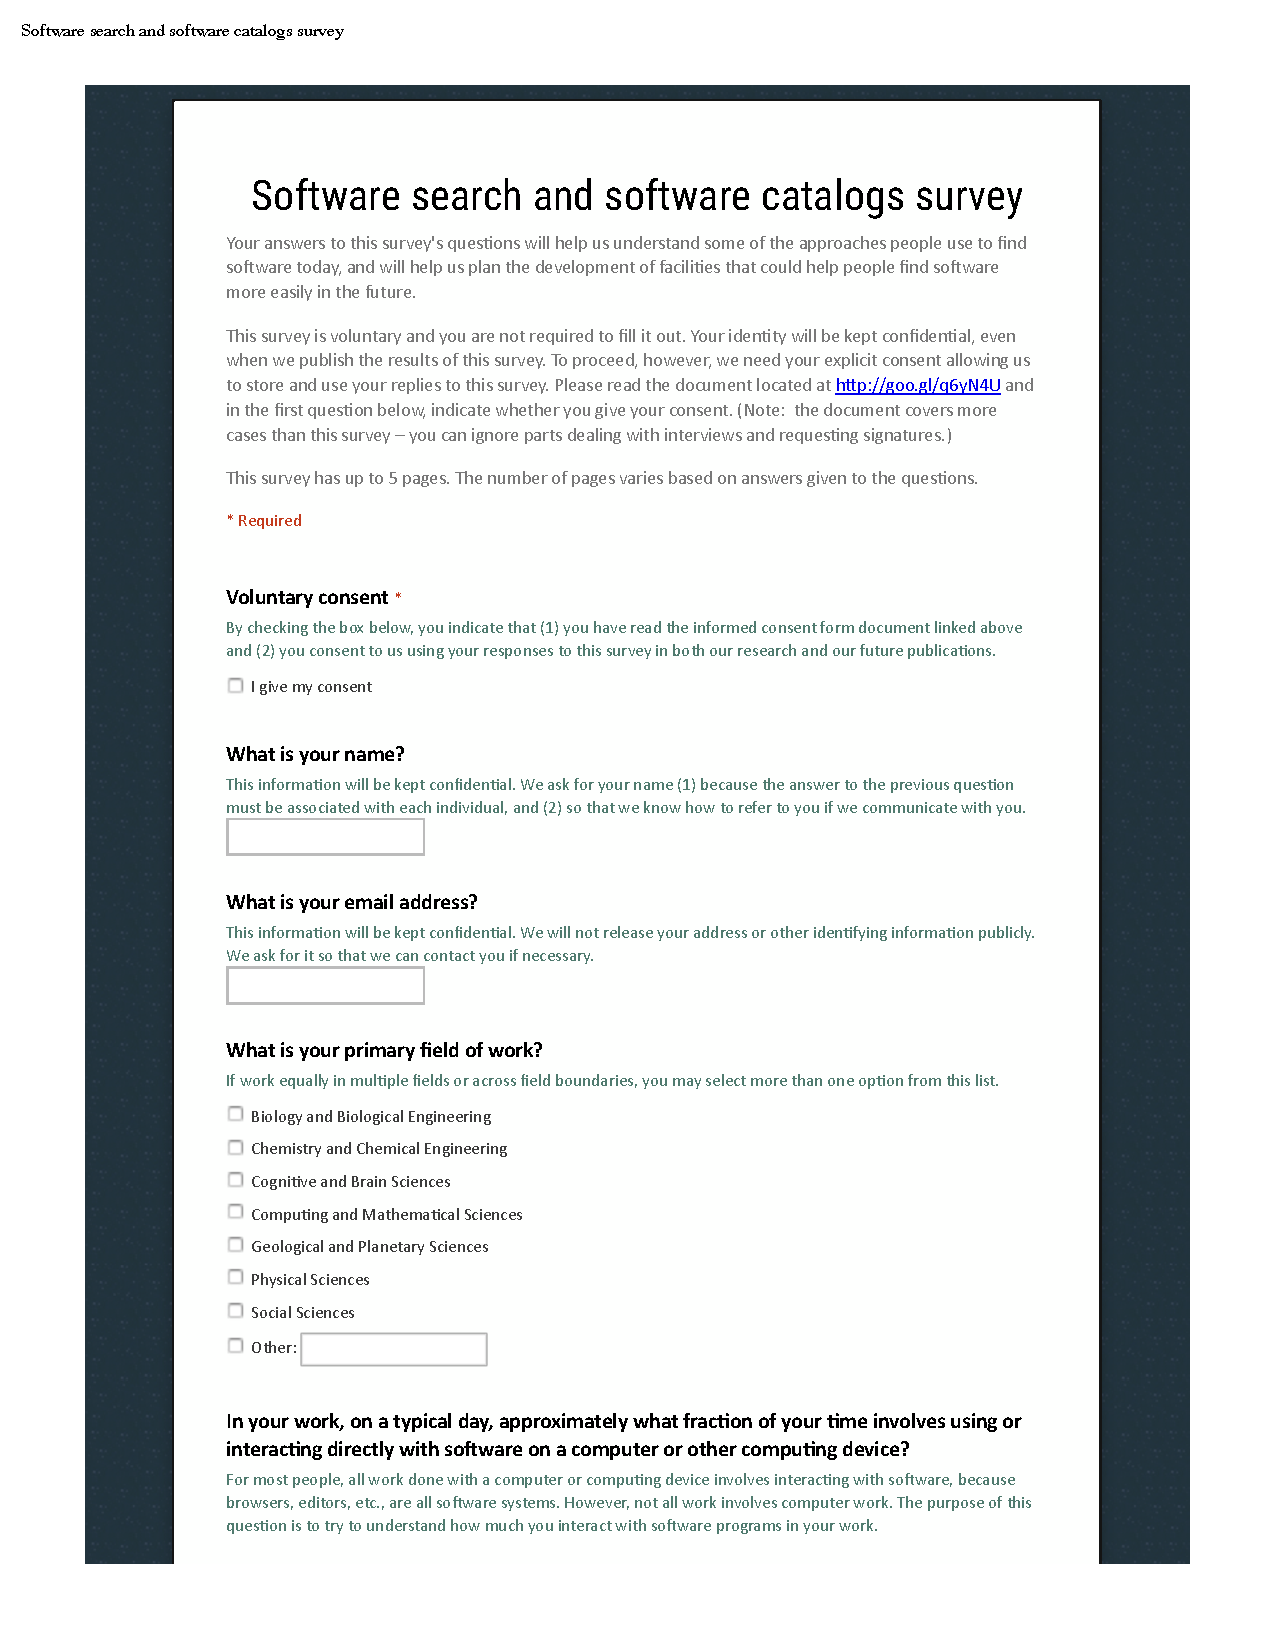
\includepdf[trim=0.25in 0.25in 0.25in 0.3in,pages={-}]{files/survey-copy/survey-2015-09-02.pdf}


\section{Invitation letters}
\label{apdx:invitations}

This section includes samples of the messages used to advertise the survey to different mailing lists and social groups.


\vspace*{2em}
\textbf{Sample Message 1}
\hrule

\small
\begin{verbatim}
Hi,

A colleague and I have been funded by NSF to do a pilot project on
"cataloging software using a semantic-based approach for software
discovery and characterization". As part of this, we are conducting an
initial survey to understand how people search for software and we would
appreciate it if you would consider taking part. The survey will take
10-15 mins and is available here:

https://goo.gl/W0jDMJ

Cheers,
\end{verbatim}
\normalsize


\vspace*{2em}
\textbf{Sample Message 2}
\hrule

\small
\begin{verbatim}
Dear colleagues,

As part of an NSF-funded project to prototype a general software
cataloguing system, we're running a survey to assess how people look for
software today (biology or otherwise).  The motivation for the effort is
simple: everyone has faced the problem of finding a suitable software tool
for a given task, and we'd like to learn more about what approaches you've
used in the past so that we can help develop better ways of finding
software in the future.  This will benefit both software users and
developers.

Here is a link to the electronic survey form:

https://goo.gl/W0jDMJ

We estimate it takes 10-15 minutes to fill out.

Best regards,
\end{verbatim}
\normalsize

% ......................................................................
\clearpage
\bibliographystyle{plainnat}
\bibliography{mike-casics-library}

\end{document}